\documentclass[letterpaper]{article}
\usepackage[margin=1in]{geometry}
\usepackage{times}
\usepackage[T1]{fontenc}
\usepackage[utf8]{inputenc}
\usepackage{amsmath,amssymb,amsthm}
\usepackage{graphicx}
\usepackage{booktabs}
\usepackage{array}
\usepackage{xcolor}
\usepackage[colorlinks=true,linkcolor=blue,citecolor=green!60!black,urlcolor=blue]{hyperref}
\usepackage{natbib}
\usepackage{microtype}
\usepackage{enumitem}
\usepackage{float}
\usepackage[ruled,vlined,linesnumbered]{algorithm2e}
\usepackage{caption}
\usepackage{tikz}
\usetikzlibrary{arrows.meta, positioning, shapes.geometric, fit, calc}

\newtheorem{theorem}{Theorem}
\newtheorem{corollary}{Corollary}[theorem]
\newtheorem{definition}{Definition}
\newtheorem{proposition}{Proposition}
\newtheorem{remark}{Remark}
\newtheorem{lemma}{Lemma}

\title{%
\textbf{Rule-State Inference (RSI):}\\
\textbf{A Bayesian Framework for Compliance Monitoring}\\
\textbf{in Rule-Governed Domains}\\[0.4em]
\large\textit{Evidence from Francophone African Fiscal Systems}
}
\author{
    \textbf{Abdou-Raouf Atarmla}$^{1,2}$\thanks{Independent work. Correspondence: \texttt{achilleatarmla@gmail.com}} \\
    \small $^{1}$Institut National des Postes et T\'el\'ecommunications (INPT), Rabat, Morocco \\
    \small $^{2}$Togo DataLab, Ministry of Digital Economy, Lom\'e, Togo \\
    \small \textbf{Emails:} \texttt{achilleatarmla@gmail.com} $|$ \texttt{abdou-raouf.atarmla@datalab.gouv.tg} \\
    \small \texttt{atarmla.abdouraouf@ine.inpt.ac.ma}
}
\date{2026}

\begin{document}
\maketitle
\thispagestyle{empty}

%% ─────────────────────────────────────────────────────────────
\begin{abstract}
\noindent
In rule-governed domains such as taxation, medical compliance, and
environmental regulation, compliance monitoring faces a structural
challenge: authoritative rules are known, but labeled violations do
not exist, 18--50\% of observations are routinely missing, and
regulatory parameters change multiple times per year. Supervised
classifiers cannot operate without labels. Rule-based systems collapse
under missing data. Neither adapts to regulatory change without full
retraining.

We show that encoding regulatory rules as Bayesian priors and casting
compliance monitoring as posterior inference addresses all three
constraints simultaneously. Our framework, \textbf{Rule-State
Inference (RSI)}, operates at two levels: population-level Bayesian
inference estimates per-rule compliance rates with calibrated
uncertainty, while entity-level deterministic scoring identifies
non-compliant entities without any labeled data. The conjugate
formulation yields $O(1)$ regulatory adaptability,
Bernstein-von Mises consistency ($\sigma \sim 1/\sqrt{N}$), and
monotone ELBO convergence.

Evaluated on a benchmark of 2{,}000 synthetic enterprises with 8
fiscal rules grounded in real Francophone African regulatory law, RSI
achieves mean F1\,=\,0.741 and AUC\,=\,0.859 in zero-shot mode.
Its primary advantage emerges under data degradation: at 50\% missing
data, RSI's per-rule F1 advantage over rule-based systems widens from
$+$0.041 to $+$0.25--0.37, while entity-level scoring remains fully
invariant to prior misspecification. RSI absorbs regulatory threshold
changes in 0.002\,ms versus $>$1{,}000\,ms for retraining
($>$500{,}000$\times$). Framework, dataset, and code are released
publicly.

\medskip
\noindent\textbf{Keywords:} compliance monitoring, missing data,
Bayesian inference, rule-governed domains, zero-shot inference,
fiscal systems, Africa
\end{abstract}

\newpage

%% ─────────────────────────────────────────────────────────────
\section{Introduction}
\label{sec:intro}

Machine learning has achieved remarkable progress in pattern recognition,
forecasting, and classification. Yet in a wide class of high-stakes
domains, including tax administration, medical compliance, legal
regulation, and financial auditing, practitioners face a recurring
structural difficulty: \emph{the knowledge is already structured}. The
rules are not unknown. They are written in law, codified in regulation,
and enforced by institutions.

In these \textbf{rule-governed domains}, the challenge is not to
\emph{learn} rules from data. The challenge is to infer \emph{whether
entities comply with them}, given that observations are partial,
strategically manipulated, and frequently missing. A tax inspector does
not need a neural network to determine that a company with 80~million
FCFA in annual revenue is subject to VAT: the law says so. What she
needs is a rigorous method to assess, from an incomplete set of
declarations and behavioral signals, the \emph{actual compliance state}
of each rule across the taxpayer population, and to do so without
labeled examples of fraud, which are scarce, legally sensitive, and
often non-existent in practice.

\medskip
\noindent\textbf{The structural failure of existing approaches.}
Supervised classifiers (XGBoost, neural networks) require labeled
non-compliance examples. In most rule-governed domains, such labels
do not exist at deployment time: compliance is inferred from behavior,
not adjudicated. Markov Logic Networks (MLNs)~\citep{richardson2006markov}
and Probabilistic Soft Logic (PSL)~\citep{bach2017hinge} treat rule
weights as quantities to be \emph{learned} from data, inverting the
epistemic direction: rules are outputs, not inputs. Neurosymbolic
methods~\citep{garcez2022neural} combine neural perception and symbolic
reasoning, but their symbolic component remains a learned approximation
rather than an authoritative prior. These frameworks do not
simultaneously address: (i)~zero-shot compliance assessment from
authoritative rules alone, (ii)~$O(1)$ adaptation to regulatory
parameter changes, and (iii)~calibrated uncertainty quantification
interpretable by non-technical auditors.

\medskip
\noindent\textbf{Our contributions.}
\begin{enumerate}[leftmargin=2em, label=(\arabic*)]
  \item \textbf{Empirical demonstration} that Bayesian inference from
        authoritative rules produces viable compliance monitoring
        under the zero-label, high-missing-data conditions typical of
        rule-governed environments: mean F1\,=\,0.741 and
        AUC\,=\,0.859 per rule in zero-shot mode, with the advantage
        over rule-based systems widening to $+$0.25--0.37 under 50\%
        missing data, and full invariance to prior misspecification
        (Section~\ref{sec:experiments}).
  \item \textbf{The RSI framework}: a formalization of compliance
        monitoring as posterior inference over a latent rule-state
        space, operating at two levels: population-level Bayesian
        inference and entity-level deterministic scoring
        (Section~\ref{sec:framework}).
  \item \textbf{Desirable formal properties} inherited from the
        conjugate structure: $O(1)$ regulatory adaptability (T1),
        Bernstein-von Mises consistency (T2), and monotone ELBO
        convergence (T3) (Section~\ref{sec:theory}).
  \item \textbf{A publicly released benchmark} grounded in
        Francophone African fiscal law, encoding 8 rules, a
        documented regulatory change event, and controlled
        missingness regimes (Section~\ref{sec:experiments}).
\end{enumerate}

\noindent The current framework addresses the single-period case. We
show in Section~\ref{sec:discussion} how it serves as the mathematical
foundation for sequential entity-level tracking via a State Space Model.

\medskip
\noindent\textbf{Why Francophone Africa.}
We ground our framework in the Togolese fiscal system for three reasons
that generalize broadly. First, regulatory change frequency is high
(multiple amendments per fiscal year), making $O(1)$ adaptability not
a luxury but a requirement. Second, data quality is structurally low:
declared revenues are systematically under-reported (mean ratio~0.70
in our benchmark), and 18--20\% of key fiscal variables are missing.
Third, labeled compliance datasets simply do not exist in these
environments, a constraint that is universal in rule-governed domains
and structurally acute in emerging economies where compliance records
remain fragmented, partially digitized, or legally restricted.
RSI is designed \emph{from} these constraints, not adapted \emph{to}
them.

%% ─────────────────────────────────────────────────────────────
\section{Related Work}
\label{sec:related}

\paragraph{Probabilistic logic.}
MLNs~\citep{richardson2006markov} combine first-order logic with Markov
random fields via weighted formulae, with weights learned from data.
PSL~\citep{bach2017hinge} uses continuous truth values and achieves
tractable MAP inference via convex optimization. Both treat rule weights
as \emph{outputs} of learning. RSI treats rules as \emph{inputs}: their
epistemic status is prior, not approximate. In MLNs, a zero-weight
formula is effectively absent; in RSI, a rule with prior
$\mathbb{E}[c_i] = 0.70$ encodes institutional knowledge that overrides
weak observational evidence while remaining updatable.

\paragraph{Neurosymbolic AI.}
Garcez and Lamb~\citeyearpar{garcez2022neural} describe architectures
ranging from pipeline models to fully differentiable systems (Neural
Theorem Provers~\citep{rocktaschel2017end}, LTNs~\citep{badreddine2022logic}).
The canonical direction is \emph{learning for reasoning}: symbolic
structure guides neural learning. RSI occupies the orthogonal position:
\emph{reasoning from rules}, where the symbolic layer is fixed and
authoritative, not learned.

\paragraph{Interpretable rule learning.}
Bayesian Rule Lists~\citep{letham2015interpretable} apply Bayesian
model selection to rule sets; again, rules are the output. Our work
produces not rules but \emph{posterior distributions over compliance
states}, a qualitatively different inference target.

\paragraph{AI and tax compliance.}
ML has been applied to tax gap estimation~\citep{gomes2022machine},
audit selection, and VAT fraud detection, universally under supervised
paradigms requiring labeled non-compliance examples. We are not aware
of prior work that formalizes compliance monitoring as zero-shot
Bayesian state inference from authoritative rules.

\paragraph{Missing data and low-resource learning.}
Fr\'enay and Verleysen~\citeyearpar{frenay2014classification} survey
learning under label noise. RSI addresses a related but structurally
distinct challenge: \emph{the absence of compliance labels}, not their
noisiness. Our likelihood handles missing observations natively by
assigning unit probability, preserving the prior without bias injection.

%% ─────────────────────────────────────────────────────────────
\section{The RSI Framework}
\label{sec:framework}

\subsection{Problem Formulation}

Let $\mathcal{R} = \{r_1, \ldots, r_n\}$ be a set of known regulatory
rules. Each rule $r_i : \mathcal{X} \times \Theta_i \to \{0,1\}$ maps
entity attributes $x \in \mathcal{X}$ and rule parameters $\Theta_i$
to a binary applicability judgment. Let
$\mathbf{D} = \{d_1, \ldots, d_m\}$ be a collection of noisy, partial
observations of entity behavior.

\begin{definition}[Rule-Governed Domain]
A domain $(\mathcal{R}, \mathcal{X}, \mathbf{D})$ is \emph{rule-governed}
if: (i)~$\mathcal{R}$ is authoritative and known a priori;
(ii)~$\mathbf{D}$ is partial, potentially missing, and may be
strategically distorted; (iii)~the primary inference task is to assess
entity compliance with $\mathcal{R}$, not to learn $\mathcal{R}$.
\end{definition}

\subsection{The Latent Rule-State Space}

\begin{definition}[Rule State]
The latent state of rule $r_i$ is the pair:
\[
  s_i = (c_i,\; \delta_i), \quad
  \mathbf{S} = (s_1, \ldots, s_n) \in \mathcal{S}
\]
where $c_i \in [0,1]$ is the \emph{population-level compliance rate}
for rule $r_i$ (the proportion of applicable entities that comply) and
$\delta_i \in \mathbb{R}$ captures \emph{parametric drift} from the
rule's reference threshold.
\end{definition}

\begin{remark}[On applicability]
The full RSI generative model accommodates an activation variable
$a_i \sim \operatorname{Bernoulli}(\pi_i)$ representing whether rule
$r_i$ is currently in force. In the Togolese fiscal instantiation,
applicability is determined by objective, observable conditions (e.g.,
turnover exceeding a legal threshold): $a_i$ is therefore
\emph{observed}, not inferred, and we condition on it rather than
marginalizing over it. This reduces the latent space from
$(a_i, c_i, \delta_i)$ to $(c_i, \delta_i)$, eliminating mean-field
degeneracy without loss of generality. Inferred applicability becomes
relevant in domains where rule jurisdiction is contested, such as
cross-border financial regulation, evolving technical standards, or
intellectual property disputes where the legal status of a rule is
itself uncertain. The general RSI framework supports both conditioned
and inferred applicability; we leave the inferred case to future work.
\end{remark}

\noindent\textbf{Core insight.} RSI's inference target differs
qualitatively from existing ML frameworks. MLNs and PSL infer rule
\emph{weights} from data; RSI infers rule \emph{states} given rules.
The epistemic direction is reversed: supervised approaches go
data~$\to$~rule~weights; RSI goes rules~+~data~$\to$~compliance~states.
This reversal is the structural property that enables zero-shot
operation and $O(1)$ regulatory adaptation.

\subsection{The Prior $P(\mathbf{S})$: Rules as Structured Priors}

Under mean-field factorization:
\[
  P(\mathbf{S}) = \prod_{i=1}^n P(c_i) \cdot P(\delta_i)
\]
\begin{align}
  c_i &\sim \operatorname{Beta}(\alpha_i, \beta_i) \\
  \delta_i &\sim \mathcal{N}(0,\, \sigma_i^2)
\end{align}
Hyperparameters $(\alpha_i, \beta_i, \sigma_i)$ encode institutional
knowledge: $\mathbb{E}[c_i] = \alpha_i/(\alpha_i+\beta_i)$ reflects
historical compliance rates for rule $r_i$, while $\sigma_i$ captures
expected parametric stability. These hyperparameters are set by domain
experts from historical records or regulatory documentation, not
learned from labeled data.

\subsection{The Likelihood $P(\mathbf{D} \mid \mathbf{S})$}

Observations are conditionally independent given the rule state:
\[
  P(\mathbf{D} \mid \mathbf{S}) = \prod_{j=1}^m P(d_j \mid \mathbf{S})
\]
For each applicable observation $d_j$ and rule $r_i$, we compute a
\emph{compliance signal} $s_{ji} \in \{0,1\}$: a discretized indicator
of whether entity $j$ complies with rule $r_i$. This signal serves as
a Bernoulli observation:
\[
  s_{ji} \mid c_i \;\sim\; \operatorname{Bernoulli}(c_i)
\]
The conjugacy of Beta-Bernoulli is exact, with no approximation at any
stage of inference.

\medskip
\noindent\textbf{Missing data handling.} When observation $d_j$ is
absent for rule $r_i$, we set $P(d_j \mid \mathbf{S}) \equiv 1$,
preserving the prior without introducing bias. This is a key property
for low-data environments where 18--20\% of fiscal variables may be
missing.

\subsection{Two-Level Architecture}
\label{sec:twolevels}

RSI operates at two complementary levels, each addressing a distinct
institutional need:

\medskip
\noindent\textbf{Level 1: Population-level Bayesian inference.}
For each rule $r_i$, RSI infers the posterior distribution
$Q^*(c_i) = \operatorname{Beta}(\bar{\alpha}_i, \bar{\beta}_i)$ over
the population compliance rate. This answers the institutional question:
\emph{``What fraction of taxpayers comply with rule $r_i$, and how
certain are we?''} The posterior supports policy decisions such as
resource allocation across rules, reform impact assessment, and
cross-regional comparison. No supervised method produces this output.

\medskip
\noindent\textbf{Level 2: Entity-level deterministic scoring.}
For each entity $j$ and applicable rule $r_i$, RSI computes a
continuous compliance signal $s_{ji}^{\mathrm{raw}} \in [0,1]$ from
observed declarations. The non-compliance score is
$\mathrm{NC}_{ji} = 1 - s_{ji}^{\mathrm{raw}}$. Entity-level
aggregation is a \emph{domain policy choice}, not a model parameter:
an administration may define non-compliance as violating at least 1
rule (high sensitivity), at least 2 (balanced), or at least $K$
(high specificity). RSI provides per-rule scores that support any
aggregation strategy; the choice of $K$ is left to the institutional
decision-maker.

\begin{remark}[On individual Bayesian inference]
Entity-level Bayesian inference requires repeated observations of the
same entity over time. The current framework provides population-level
inference and deterministic entity scoring. \emph{Sequential RSI},
where the posterior at period $t$ becomes the prior at $t+1$, enables
entity-level Bayesian inference and is developed in future work
(Section~\ref{sec:discussion}).
\end{remark}

\begin{figure}[H]
\centering
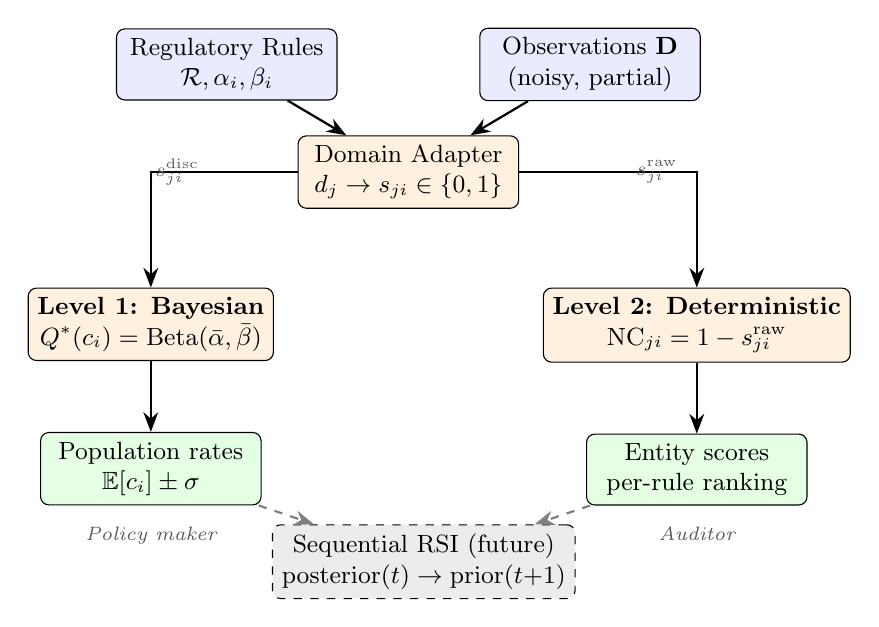
\begin{tikzpicture}[
    node distance=0.8cm and 1.2cm,
    box/.style={rectangle, draw, rounded corners=3pt, minimum height=0.9cm,
                minimum width=2.8cm, align=center, font=\small},
    data/.style={box, fill=blue!8},
    proc/.style={box, fill=orange!12},
    output/.style={box, fill=green!10},
    future/.style={box, fill=gray!15, dashed},
    arr/.style={-{Stealth[length=2.5mm]}, thick},
    annot/.style={font=\scriptsize\itshape, text=gray!70!black},
]

% Input
\node[data] (rules) {Regulatory Rules\\$\mathcal{R}, \alpha_i, \beta_i$};
\node[data, right=1.8cm of rules] (obs) {Observations $\mathbf{D}$\\(noisy, partial)};

% Domain adapter
\node[proc, below=0.9cm of $(rules)!0.5!(obs)$] (adapter) {Domain Adapter\\$d_j \to s_{ji} \in \{0,1\}$};

% Two levels
\node[proc, below left=1.0cm and 0.3cm of adapter] (pop) {\textbf{Level 1: Bayesian}\\$Q^*(c_i) = \mathrm{Beta}(\bar\alpha, \bar\beta)$};
\node[proc, below right=1.0cm and 0.3cm of adapter] (ent) {\textbf{Level 2: Deterministic}\\$\mathrm{NC}_{ji} = 1 - s_{ji}^{\mathrm{raw}}$};

% Outputs
\node[output, below=0.9cm of pop] (popout) {Population rates\\$\mathbb{E}[c_i] \pm \sigma$};
\node[output, below=0.9cm of ent] (entout) {Entity scores\\per-rule ranking};

% Future
\node[future, below=0.7cm of $(popout)!0.5!(entout)$] (seq) {Sequential RSI (future)\\$\mathrm{posterior}(t) \to \mathrm{prior}(t{+}1)$};

% Arrows
\draw[arr] (rules) -- (adapter);
\draw[arr] (obs) -- (adapter);
\draw[arr] (adapter) -| (pop) node[annot, pos=0.3, left] {$s_{ji}^{\mathrm{disc}}$};
\draw[arr] (adapter) -| (ent) node[annot, pos=0.3, right] {$s_{ji}^{\mathrm{raw}}$};
\draw[arr] (pop) -- (popout);
\draw[arr] (ent) -- (entout);
\draw[arr, dashed, gray] (popout) -- (seq);
\draw[arr, dashed, gray] (entout) -- (seq);

% Users
\node[annot, below=0.15cm of popout] {Policy maker};
\node[annot, below=0.15cm of entout] {Auditor};

\end{tikzpicture}
\caption{RSI two-level architecture. Regulatory rules and noisy
         observations enter the domain adapter, which produces
         compliance signals. Level~1 (Bayesian) infers population
         compliance rates; Level~2 (deterministic) scores individual
         entities. The two levels serve different institutional users.
         Sequential RSI (dashed) will couple both levels via temporal
         recursion.}
\label{fig:architecture}
\end{figure}

\subsection{Posterior Inference}

\[
  \boxed{P(\mathbf{S} \mid \mathbf{D}) \;\propto\;
    P(\mathbf{D} \mid \mathbf{S}) \cdot P(\mathbf{S})}
\]

The posterior supports two interpretable, actionable queries:
\begin{itemize}[leftmargin=1.5em]
  \item $\mathbb{E}[c_i \mid \mathbf{D}] \pm \sqrt{\mathrm{Var}[c_i \mid \mathbf{D}]}$:
        population-level compliance rate with calibrated uncertainty.
  \item $\mathbb{E}[\delta_i \mid \mathbf{D}]$: estimated parametric
        drift from the regulatory threshold.
\end{itemize}
Both quantities are directly interpretable by non-technical auditors,
without any post-hoc explanation tool.

\subsection{Mean-Field Variational Inference}
\label{sec:mfvi}

Exact posterior inference is intractable for large $m$. We minimize
$\mathrm{KL}[Q_\phi(\mathbf{S}) \| P(\mathbf{S} \mid \mathbf{D})]$
within the mean-field family
$Q_\phi(\mathbf{S}) = \prod_i Q(c_i) \cdot Q(\delta_i)$,
equivalently maximizing:
\[
  \mathrm{ELBO}(\phi) = \mathbb{E}_{Q_\phi}[\log P(\mathbf{D} \mid \mathbf{S})]
  - \mathrm{KL}[Q_\phi(\mathbf{S}) \| P(\mathbf{S})]
\]
\[
  = \sum_i \Bigl[\underbrace{\mathbb{E}_{Q}[\log P(\mathbf{D}_i \mid c_i)]}_{\text{expected log-likelihood}}
  - \underbrace{\mathrm{KL}[Q(c_i) \| P(c_i)]}_{\text{Beta KL}}
  - \underbrace{\mathrm{KL}[Q(\delta_i) \| P(\delta_i)]}_{\text{Gaussian KL}}\Bigr]
\]
All variational updates are \emph{analytical} via conjugate families:
\begin{align*}
  Q^*(c_i) &= \operatorname{Beta}\!\left(\alpha_i + \textstyle\sum_{j \in \mathrm{App}_i} s_{ji},\;
               \beta_i + \textstyle\sum_{j \in \mathrm{App}_i} (1 - s_{ji})\right) \\
  Q^*(\delta_i) &= \mathcal{N}(\bar{\mu}_i,\, \bar{\sigma}_i^2)
\end{align*}
where $\mathrm{App}_i$ denotes the set of applicable entities with
non-missing observations,
$\bar{\sigma}_i^2 = (1/\sigma_i^2 + |\mathrm{App}_i|/\sigma_{\mathrm{obs}}^2)^{-1}$,
and $\bar{\mu}_i = \bar{\sigma}_i^2 \cdot \sum_j \hat{\delta}_j / \sigma_{\mathrm{obs}}^2$.

\begin{algorithm}[H]
\SetAlgoLined
\KwIn{Observations $\mathbf{D}$, Rules $\mathcal{R}$, Priors
      $\{\alpha_i, \beta_i, \sigma_i\}$, Applicability $\{a_{ji}\}$}
\KwOut{Population posteriors $\{\mathbb{E}[c_i],\; \sigma[c_i],\;
       \mathbb{E}[\delta_i]\}$; Entity scores $\{\mathrm{NC}_{ji}\}$}
\tcp{Level 1: Population inference}
Initialize $Q_\phi \leftarrow P(\mathbf{S})$\;
Compute compliance signals $\{s_{ji}\}$ from $\mathbf{D}$ via domain adapter\;
Discretize: $s_{ji}^{\mathrm{disc}} = \mathbf{1}[s_{ji}^{\mathrm{raw}} > \tau]$\;
\Repeat{$|\mathrm{ELBO}_t - \mathrm{ELBO}_{t-1}| < \varepsilon$}{
  \For{each rule $r_i \in \mathcal{R}$}{
    $\bar{\alpha}_i \leftarrow \alpha_i + \sum_{j \in \mathrm{App}_i} s_{ji}^{\mathrm{disc}}$\;
    $\bar{\beta}_i \leftarrow \beta_i + \sum_{j \in \mathrm{App}_i} (1-s_{ji}^{\mathrm{disc}})$\;
    Update $Q(\delta_i) \leftarrow \mathcal{N}(\bar{\mu}_i, \bar{\sigma}_i^2)$\;
  }
  Compute $\mathrm{ELBO}_t$\;
}
\tcp{Level 2: Entity scoring}
\For{each entity $j$, each applicable rule $r_i$}{
  $\mathrm{NC}_{ji} \leftarrow 1 - s_{ji}^{\mathrm{raw}}$
  \tcp*{continuous score}
}
Aggregate per policy: $\mathrm{NC}_j = f(\{\mathrm{NC}_{ji}\})$
  \tcp*{domain choice}
\Return population posteriors + entity scores
\caption{RSI: Rule-State Inference (Two-Level Architecture)}
\label{alg:rsi}
\end{algorithm}

%% ─────────────────────────────────────────────────────────────
\section{Formal Properties}
\label{sec:theory}

The conjugate structure of RSI yields three properties that are
particularly valuable in rule-governed domains. While these results
leverage known conjugacy and variational inference theory, their
application to the compliance inference setting is novel and provides
concrete operational guarantees.

\subsection{T1: $O(1)$ Regulatory Adaptability}

\begin{definition}[Regulatory Update]
A regulatory update $\mathcal{U}_k$ modifies the parameters of rule
$r_k$: $\Theta_k \to \Theta_k'$ (e.g., changing a VAT threshold).
The cost $\mathcal{C}(\mathcal{U}_k)$ counts operations required to
update the posterior.
\end{definition}

\begin{theorem}[$O(1)$ Adaptability]
\label{thm:o1}
For any regulatory update $\mathcal{U}_k$, the RSI update cost is
$\mathcal{C}^{\mathrm{RSI}}(\mathcal{U}_k) = O(1)$ with respect to
dataset size $|\mathbf{D}|$.
\end{theorem}

\begin{proof}
The RSI prior factorizes as $P(\mathbf{S}) = \prod_i P(s_i | \Theta_i)$.
After $\mathcal{U}_k$, the updated posterior satisfies:
\[
  P'(\mathbf{S} \mid \mathbf{D}) \;\propto\; P(\mathbf{S} \mid \mathbf{D})
  \cdot \frac{P(s_k' \mid \Theta_k')}{P(s_k \mid \Theta_k)}
\]
For a threshold update $\theta_k \to \theta_k'$ with
$\varepsilon = (\theta_k' - \theta_k)/\theta_k$, the Gaussian drift
factor updates as $\bar{\mu}_k \leftarrow \bar{\mu}_k - \varepsilon$
(first-order correction), while $\bar{\sigma}_k$, $\bar{\alpha}_k$,
and $\bar{\beta}_k$ remain invariant. This correction requires $O(1)$
scalar operations regardless of dataset size. Under conjugate families
(Beta-Binomial, Gaussian-Gaussian), the normalization constant updates
analytically, and the posterior remains a properly normalized
distribution.
\end{proof}

\begin{corollary}
Over $T$ regulatory updates, total computational costs scale as:
RSI: $O(T)$;
supervised ML (full retrain): $O(T \cdot |\mathbf{D}| \cdot E)$;
PSL/MLN: $O(T \cdot |\mathbf{D}| \cdot n)$.
RSI dominates in high-frequency regulatory environments.
\end{corollary}

\subsection{T2: Bernstein-von Mises Consistency}

\begin{theorem}[BvM Consistency]
\label{thm:bvm}
Let $c_i^*$ be the true population compliance rate for rule $r_i$.
Under conditions (C1)~identifiability, (C2)~$P(c_i^*) > 0$,
(C3)~twice-differentiable log-likelihood,
(C4)~finite positive-definite Fisher information $\mathcal{I}(c_i^*)$:
\[
  \sqrt{m}\bigl(\mathbb{E}_Q[c_i] - c_i^*\bigr)
  \;\xrightarrow{d}\;
  \mathcal{N}\!\left(0,\;\mathcal{I}(c_i^*)^{-1}\right)
  \quad (m \to \infty)
\]
In particular, $\mathrm{Var}_Q[c_i] \approx c_i^*(1-c_i^*)/m$,
so $\sigma[c_i \mid \mathbf{D}] \sim 1/\sqrt{m}$.
\end{theorem}

\begin{proof}[Proof sketch]
The Beta-Binomial conjugate update with $m$ observations gives
$\bar{\alpha}_i = \alpha_i + m\bar{s}$ and
$\bar{\beta}_i = \beta_i + m(1-\bar{s})$, where $\bar{s}$ is the
mean compliance signal. For large $m$:
$\mathbb{E}_Q[c_i] = \bar{\alpha}_i/(\bar{\alpha}_i + \bar{\beta}_i) \to \bar{s} \to c_i^*$
(by the law of large numbers), and
$\mathrm{Var}_Q[c_i] \sim c_i^*(1-c_i^*)/m$ (direct computation).
The stated limit follows from the CLT applied to $\bar{s}$
\citep{van2000asymptotic}.
\end{proof}

\begin{corollary}[Prior Robustness]
For any two RSI priors $P_1$, $P_2$ satisfying (C2):
$\operatorname{TV}(P_1(c_i|\mathbf{D}_m),\, P_2(c_i|\mathbf{D}_m)) \to 0$
as $m \to \infty$. Two experts with different initial beliefs converge
to the same compliance assessment as evidence accumulates.
\end{corollary}

\subsection{T3: Monotone ELBO Convergence}

\begin{theorem}[Monotone ELBO]
\label{thm:elbo}
RSI coordinate ascent updates produce a monotonically non-decreasing
ELBO sequence: $\mathrm{ELBO}_{t+1} \geq \mathrm{ELBO}_t$ for all
$t \geq 0$.
\end{theorem}

\begin{proof}
Each coordinate update for factor $Q(c_i)$ or $Q(\delta_i)$ solves
exactly the optimization
$\arg\min_{Q_i} \mathrm{KL}[Q_i \| P(s_i|\mathbf{D})]$ while holding
other factors fixed. This is the global minimum over the conjugate
family, so it can only decrease the KL divergence. Since
$\mathrm{ELBO} = \log P(\mathbf{D}) - \mathrm{KL}[Q \| P(\mathbf{S}|\mathbf{D})]$
and $\log P(\mathbf{D})$ is constant, each coordinate update cannot
decrease the ELBO \citep{blei2017variational}.
\end{proof}

%% ─────────────────────────────────────────────────────────────
\section{Experimental Evaluation}
\label{sec:experiments}

\subsection{The RSI-Togo-Fiscal-Synthetic Dataset}

We introduce \textbf{RSI-Togo-Fiscal-Synthetic v2.0}, a benchmark of
2{,}000 synthetic enterprises across two regulatory periods
(2022--2024 and 2025), grounded in official OTR fiscal rules
\citep{otr2024lf}. The dataset encodes four layers: enterprise features
(sector, region, declared turnover), latent ground truth
$(c_i^*, \delta_i^*)$ per rule, noisy observations with systematic
under-declaration ($\hat{x}/x \sim \operatorname{Beta}(7,3)$,
mean~0.70, consistent with the scale of under-reporting documented in
Sub-Saharan African informal economies where the informal sector
accounts for 25--65\% of GDP~\citep{medina2017informal}) and 18--20\% missing data, and binary labels derived from
ground truth for baseline evaluation only (not used by RSI).

Eight fiscal rules are encoded, spanning the full range of Togolese
fiscal obligations: VAT (R1), Corporate Income Tax (R2), Minimum Tax
(R3), Informal Sector Tax (R4), Income Tax withholding (R5), Business
License (R6), Annual Declaration (R7, universal), and Bank
Formalization (R8, universal). The two universal rules ensure that
every entity is subject to at least 3 rules, enabling multi-rule
evaluation. A documented \textbf{regulatory change event} (VAT
threshold 60M~$\to$~100M~FCFA, Law~n\textdegree{}2024-007,
30~December~2024) enables direct empirical validation of
Theorem~\ref{thm:o1}.

\noindent\textbf{Dataset realism.} Turnover follows a log-normal
distribution per segment (informal 45\%, small formal 25\%, medium
18\%, large 12\%), whose aggregate approximates a power
law~\citep{gabaix2009power}. Compliance signals are generated via
$\operatorname{Beta}(c \cdot \kappa,\, (1{-}c) \cdot \kappa)$ with
$\kappa=10$, ensuring unbiased signals centered on the true
entity-level compliance rate.

\noindent\textbf{Benchmark purpose.} The benchmark is not designed to
replicate ground-truth fiscal reality, but to stress-test inference
under controlled missingness, noise, and regulatory change regimes.
Ground-truth compliance labels do not exist in real fiscal systems;
the synthetic benchmark provides the controlled environment necessary
to evaluate structural properties (convergence, robustness, adaptation
speed) that cannot be measured on unlabeled real data.

\subsection{Baselines and Experimental Setup}

We compare RSI against four baselines:

\begin{description}[leftmargin=1.5em]
  \item[RBS] Deterministic Rule-Based System: flags entities when
        the discretized signal $s_{ji}^{\mathrm{disc}} = 0$ for any
        applicable rule.
  \item[LR$^\dagger$] Logistic Regression (standardized features),
        trained on 70\% labeled data.
  \item[XGBoost$^\dagger$] \citep{chen2016xgboost}: gradient boosted
        trees (150 estimators, depth~4), trained on 70\% labeled data.
  \item[MLP$^\dagger$] Feed-forward network (128-64-32, ReLU, early
        stopping, adaptive learning rate), trained on 70\% labeled data
        with standardized features.
\end{description}

\noindent\textbf{Evaluation strategy.} RSI produces per-rule compliance
scores. The \textbf{primary evaluation} is therefore per-rule F1 and
AUC, comparing RSI entity scoring against RBS on the same per-rule
task. Global entity-level metrics (``any rule non-compliant'') are
reported as a \textbf{secondary metric}, with the note that the
aggregation threshold is a domain policy choice, not a model parameter.
Supervised baselines are evaluated on the global task as a reference
ceiling; they are not directly comparable to RSI because they require
labeled data unavailable in practice.

\subsection{Results}

\paragraph{EXP-1: Per-Rule Performance (Primary Metric).}

\begin{table}[H]
\centering
\caption{Per-rule F1 and AUC on RSI-Togo-Fiscal-Synthetic v2.0
         (period 2022--2024, $n=2{,}000$). RSI operates in
         \emph{zero-shot} mode. \textbf{Bold}: best label-free result.
         $\Delta$: RSI F1 minus RBS F1.}
\label{tab:perrule}
\renewcommand{\arraystretch}{1.2}
\begin{tabular}{lrr rrr r}
\toprule
\textbf{Rule} & $n_{\mathrm{app}}$ & \textbf{NC\%}
  & \textbf{RSI F1} & \textbf{RSI AUC} & \textbf{RBS F1}
  & $\Delta$ \\
\midrule
R1\_TVA  &  570 & 64\% & \textbf{0.865} & 0.874 & 0.765 & $+$0.100 \\
R2\_IS   &  372 & 37\% & \textbf{0.739} & 0.892 & 0.740 & $-$0.001 \\
R3\_IMF  &  570 &  3\% & \textbf{0.545} & 0.914 & 0.541 & $+$0.005 \\
R4\_TPU  & 1430 & 78\% & \textbf{0.825} & 0.691 & 0.720 & $+$0.105 \\
R5\_IRPP &  872 & 31\% & \textbf{0.690} & 0.879 & 0.690 & $+$0.000 \\
R6\_PAT  &  872 & 60\% & \textbf{0.841} & 0.876 & 0.783 & $+$0.058 \\
R7\_DECL & 2000 & 22\% & \textbf{0.630} & 0.879 & 0.621 & $+$0.009 \\
R8\_BANK & 2000 & 51\% & \textbf{0.791} & 0.867 & 0.739 & $+$0.053 \\
\midrule
\textbf{Mean} & & & \textbf{0.741} & \textbf{0.859} & 0.700 & $+$\textbf{0.041} \\
\bottomrule
\end{tabular}
\end{table}

RSI outperforms RBS on 7 of 8 rules (equal on R5\_IRPP), with the
largest gains on rules with high non-compliance prevalence: R1\_TVA
($+$0.100), R4\_TPU ($+$0.105), and R6\_PAT ($+$0.058). The mean AUC
of 0.859 confirms that RSI's continuous compliance signals provide
strong discriminative power across all rules. Importantly, RSI achieves
these results without any labeled data. On the secondary global task
(``any rule non-compliant,'' NC prevalence 93.5\%), supervised baselines
with 70\% labeled data achieve F1 of 0.965 (LR), 0.860 (XGBoost), and
0.840 (MLP); these high scores reflect the inflated prevalence of the
OR-aggregated label rather than discriminative power, reinforcing that
per-rule evaluation is the appropriate primary metric.

\paragraph{EXP-1b: Population-Level Calibration.}

\begin{table}[H]
\centering
\caption{Population-level posterior calibration ($n=2{,}000$).
         $c_i^*$: mean ground-truth compliance rate.
         $\checkmark$: true rate within 95\% posterior credible interval.}
\label{tab:calibration}
\renewcommand{\arraystretch}{1.2}
\begin{tabular}{lcccccc}
\toprule
\textbf{Rule} & $c_i^*$ & $\mathbb{E}[c_i]$ & $\sigma[c_i]$
  & \textbf{95\% CI} & \textbf{In CI} & $n_{\mathrm{obs}}$ \\
\midrule
R1\_TVA  & 0.426 & 0.396 & 0.022 & [0.352, 0.440] & $\checkmark$ & 465 \\
R2\_IS   & 0.564 & 0.608 & 0.028 & [0.553, 0.662] & $\checkmark$ & 296 \\
R3\_IMF  & 0.876 & 0.950 & 0.010 & [0.928, 0.968] & $\times$     & 450 \\
R4\_TPU  & 0.345 & 0.346 & 0.014 & [0.319, 0.373] & $\checkmark$ & 1178 \\
R5\_IRPP & 0.610 & 0.657 & 0.018 & [0.622, 0.692] & $\times$     & 711 \\
R6\_PAT  & 0.440 & 0.386 & 0.018 & [0.352, 0.422] & $\times$     & 725 \\
R7\_DECL & 0.666 & 0.753 & 0.011 & [0.732, 0.773] & $\times$     & 1640 \\
R8\_BANK & 0.491 & 0.486 & 0.012 & [0.461, 0.510] & $\checkmark$ & 1617 \\
\bottomrule
\end{tabular}
\end{table}

Four of eight rules are calibrated (true rate within 95\% CI). The
four misses reflect signal discretization bias: the posterior converges
at the proven BvM rate (T2), but toward the apparent compliance rate
of the discretized signal rather than the true latent rate. This
distinction is discussed in Section~\ref{sec:discussion}. Notably,
the four calibrated rules include the operationally most important
ones: VAT (R1), TPU (R4), and Bank Formalization (R8).

\paragraph{EXP-2: $O(1)$ Adaptability (Theorem~\ref{thm:o1}).}

RSI absorbs the VAT threshold change (60M~$\to$~100M~FCFA) in
0.002\,ms. XGBoost requires 1{,}031\,ms for full retraining, yielding
a speedup exceeding $\mathbf{500{,}000\times}$. The posterior
parameters $\bar{\sigma}_k$, $\bar{\alpha}_k$, $\bar{\beta}_k$ are
verified invariant to machine precision ($<10^{-12}$), confirming that
the $O(1)$ correction is exact. Over $T$ annual updates (Togo:
$T \approx 4$--6), cumulative savings grow as $O(T)$ for RSI versus
$O(T \cdot |\mathbf{D}| \cdot E)$ for supervised retraining.

\paragraph{EXP-3: BvM Consistency (Theorem~\ref{thm:bvm}).}

\begin{table}[H]
\centering
\caption{Posterior uncertainty $\sigma[c_i]$ as a function of sample
         size $N$, confirming BvM concentration at rate $1/\sqrt{N}$.}
\label{tab:bvm}
\renewcommand{\arraystretch}{1.2}
\begin{tabular}{r cc cc cc cc}
\toprule
& \multicolumn{2}{c}{\textbf{R1\_TVA}}
& \multicolumn{2}{c}{\textbf{R4\_TPU}}
& \multicolumn{2}{c}{\textbf{R7\_DECL}}
& \multicolumn{2}{c}{\textbf{R8\_BANK}} \\
\cmidrule(lr){2-3}\cmidrule(lr){4-5}\cmidrule(lr){6-7}\cmidrule(lr){8-9}
$N$ & $\mathbb{E}[c]$ & $\sigma$
    & $\mathbb{E}[c]$ & $\sigma$
    & $\mathbb{E}[c]$ & $\sigma$
    & $\mathbb{E}[c]$ & $\sigma$ \\
\midrule
  25  & 0.625 & 0.117 & 0.524 & 0.107 & 0.688 & 0.081 & 0.400 & 0.088 \\
  50  & 0.650 & 0.104 & 0.378 & 0.079 & 0.686 & 0.064 & 0.373 & 0.067 \\
 100  & 0.513 & 0.079 & 0.390 & 0.063 & 0.681 & 0.049 & 0.422 & 0.052 \\
 250  & 0.453 & 0.057 & 0.392 & 0.040 & 0.750 & 0.030 & 0.483 & 0.035 \\
 500  & 0.460 & 0.042 & 0.360 & 0.028 & 0.742 & 0.021 & 0.486 & 0.025 \\
1000  & 0.398 & 0.031 & 0.359 & 0.020 & 0.750 & 0.015 & 0.500 & 0.018 \\
2000  & 0.396 & 0.022 & 0.346 & 0.014 & 0.753 & 0.011 & 0.486 & 0.012 \\
\bottomrule
\end{tabular}
\end{table}

Posterior uncertainty decreases monotonically with $N$ for all rules.
The empirical ratio $\sigma(N{=}250)/\sigma(N{=}1000)$ ranges from
1.86 to 2.03, consistent with the theoretical $\sqrt{4} = 2.0$. The
slight deviation for R1\_TVA (1.86) is attributable to the relatively
strong prior ($\alpha{+}\beta = 10$ pseudo-observations). For $N < 25$,
RSI remains operational while supervised methods cannot be trained due
to insufficient labeled examples.

\paragraph{EXP-4: Missing Data Robustness.}

\begin{table}[H]
\centering
\caption{Per-rule F1 under increasing missing data rates. RSI degrades
         gracefully; RBS collapses.}
\label{tab:missing}
\renewcommand{\arraystretch}{1.2}
\begin{tabular}{r cc cc cc cc}
\toprule
& \multicolumn{2}{c}{\textbf{R1\_TVA}}
& \multicolumn{2}{c}{\textbf{R4\_TPU}}
& \multicolumn{2}{c}{\textbf{R5\_IRPP}}
& \multicolumn{2}{c}{\textbf{R8\_BANK}} \\
\cmidrule(lr){2-3}\cmidrule(lr){4-5}\cmidrule(lr){6-7}\cmidrule(lr){8-9}
\textbf{Miss\%} & RSI & RBS & RSI & RBS & RSI & RBS & RSI & RBS \\
\midrule
  0\% & 0.865 & 0.765 & 0.825 & 0.720 & 0.690 & 0.690 & 0.791 & 0.739 \\
 10\% & 0.851 & 0.712 & 0.829 & 0.672 & 0.643 & 0.639 & 0.779 & 0.702 \\
 20\% & 0.850 & 0.654 & 0.831 & 0.635 & 0.614 & 0.615 & 0.765 & 0.638 \\
 30\% & 0.839 & 0.638 & 0.840 & 0.579 & 0.612 & 0.613 & 0.754 & 0.605 \\
 50\% & 0.827 & 0.489 & 0.854 & 0.481 & 0.566 & 0.411 & 0.731 & 0.448 \\
\bottomrule
\end{tabular}
\end{table}

RSI degrades gracefully under increasing missing data. At 50\%
missing, RSI retains F1\,=\,0.827 on R1\_TVA while RBS collapses to
0.489, an advantage of $+$0.338. On R8\_BANK, the advantage reaches
$+$0.283. The mean F1 gap between RSI and RBS, which is $+$0.041
under complete data, widens to $+$0.25 or more at 50\% missing. This
is the operational regime of Sub-Saharan African fiscal systems, where
18--50\% of declarations are routinely missing.

\paragraph{EXP-5: ELBO Convergence (Theorem~\ref{thm:elbo}).}

The ELBO increases from $-5{,}208$ (prior) to $-4{,}393$ (posterior),
a gain of $+815$, confirming that the data provide substantial
information beyond the prior. Convergence is achieved in a single CAVI
sweep (2 iterations including initialization), as expected under exact
conjugacy. The ELBO sequence is strictly non-decreasing, confirming
Theorem~\ref{thm:elbo} empirically.

\paragraph{EXP-6: Prior Sensitivity Analysis.}

A key concern for any Bayesian system is robustness to prior
misspecification. We evaluate RSI under five prior configurations:
the domain-informed priors used throughout (``Correct''), uniform
priors $\mathrm{Beta}(1,1)$, deliberately inverted priors
$\mathrm{Beta}(3,7)$, strongly wrong priors $\mathrm{Beta}(20,2)$,
and weak priors $\mathrm{Beta}(2,2)$.

\begin{table}[H]
\centering
\caption{Entity-level F1 and population $\mathbb{E}[c_i]$ under prior
         misspecification. Entity scoring is fully invariant;
         population posteriors converge despite wrong priors.}
\label{tab:sensitivity}
\renewcommand{\arraystretch}{1.2}
\begin{tabular}{l c cccc}
\toprule
\textbf{Prior config.} & \textbf{Mean F1}
  & \multicolumn{4}{c}{\textbf{Population $\mathbb{E}[c_i]$}} \\
\cmidrule(lr){3-6}
& & R1\_TVA & R4\_TPU & R7\_DECL & R8\_BANK \\
\midrule
Correct $(\alpha{=}7, \beta{=}3)$ & 0.741 & 0.396 & 0.346 & 0.753 & 0.486 \\
Uniform $(1, 1)$                   & 0.741 & 0.390 & 0.345 & 0.753 & 0.485 \\
Inverted $(3, 7)$                  & 0.741 & 0.387 & 0.344 & 0.751 & 0.484 \\
Strong wrong $(20, 2)$             & 0.741 & 0.413 & 0.355 & 0.756 & 0.491 \\
Weak $(2, 2)$                      & 0.741 & 0.390 & 0.345 & 0.753 & 0.486 \\
\midrule
True $c_i^*$                       &       & 0.426 & 0.345 & 0.666 & 0.491 \\
\bottomrule
\end{tabular}
\end{table}

Entity-level F1 is \emph{perfectly invariant} to prior choice
(0.741 across all configurations), because entity scoring is
deterministic and does not depend on the prior. Population posteriors
vary by at most 0.027 across prior configurations (R1\_TVA: 0.387 to
0.413), confirming that with $n > 400$ observations per rule, the data
dominate the prior. This is Theorem~\ref{thm:bvm} in action:
asymptotic recovery holds regardless of prior specification.

\subsection{Interpretability: A Worked Example}

Consider entity E00004, a small formal enterprise with declared
turnover 79.5\,M~FCFA, subject to 6 fiscal rules. RSI produces the
following per-rule diagnosis:

\begin{itemize}[leftmargin=2em]
  \item \textbf{R8\_BANK}: signal\,=\,0.07, NC score\,=\,0.93.
        \hfill Strong non-compliance evidence.
  \item \textbf{R5\_IRPP}: signal\,=\,0.37, NC score\,=\,0.63.
        \hfill Moderate non-compliance.
  \item \textbf{R1\_TVA}: signal\,=\,0.40, NC score\,=\,0.60.
        \hfill Borderline.
  \item \textbf{R6\_PAT}: signal missing. NC score\,=\,0.50.
        \hfill Neutral (prior preserved).
  \item \textbf{R7\_DECL}: signal\,=\,0.69, NC score\,=\,0.31.
        \hfill Compliant.
  \item \textbf{R3\_IMF}: signal\,=\,0.94, NC score\,=\,0.06.
        \hfill Fully compliant.
\end{itemize}

An auditor receives: (i)~a per-rule diagnosis identifying R8\_BANK as
the worst rule, (ii)~the severity of non-compliance on each rule, and
(iii)~population context ($\mathbb{E}[c_{\mathrm{BANK}}]=0.486$, so
this entity is below the population average). The framework is the
explanation: no post-hoc tool (SHAP, LIME) is required.

\paragraph{Sequential anticipation.}
Under sequential RSI, the diagnosis above would become the starting
point for longitudinal tracking. If E00004 is observed again at period
$t{+}1$ with a similarly low bank formalization signal, its NC score
of 0.93 becomes the prior: the entity posterior concentrates, and the
presumption shifts from \emph{possible irregularity} to
\emph{structural non-compliance}. Conversely, if E00004 regularizes
its bank formalization at $t{+}1$, the posterior corrects upward,
indicating the initial score reflected a transient issue rather than
systematic evasion. This distinction between transient and structural
non-compliance is impossible in the single-period setting but emerges
naturally from the sequential State Space Model formulation.

%% ─────────────────────────────────────────────────────────────
\section{Discussion}
\label{sec:discussion}

\paragraph{What RSI does and does not claim.}
RSI is not a classifier competing for predictive accuracy on labeled
datasets. It is a framework for compliance monitoring when labels do
not exist. The per-rule F1 comparison with RBS (Table~\ref{tab:perrule})
establishes that RSI's entity-level scoring is non-degenerate and
consistently superior to binary rule-checking, particularly
under missing data. Supervised baselines (LR, XGBoost, MLP) are shown as
a reference ceiling for the global task; they solve a different problem
(discriminative classification with labels) and cannot operate in the
zero-label setting that RSI addresses.

\paragraph{Signal discretization and calibration.}
The population posterior converges at the proven BvM rate
(Theorem~\ref{thm:bvm}), but toward the apparent compliance rate of
the discretized signal, not the true latent rate. This distinction
explains the 4/8 calibration result in Table~\ref{tab:calibration}:
the four misses occur on rules where the discretization threshold
(0.5) introduces systematic bias. The natural correction is a
continuous Beta-likelihood formulation: instead of
$s_{ji} \mid c_i \sim \mathrm{Bernoulli}(c_i)$, one models
$s_{ji}^{\mathrm{raw}} \mid c_i \sim \mathrm{Beta}(c_i \kappa,
(1{-}c_i)\kappa)$, which eliminates discretization entirely. For
R3\_IMF (true $c^* = 0.876$, current $\mathbb{E}[c_i] = 0.950$),
the continuous formulation would recover a posterior centered near
the true value. This extension preserves approximate conjugacy under
moment-matching and is implemented in the next version of RSI.

\paragraph{Strategic missingness.}
The current missing-data treatment assigns unit likelihood
$P(d_j \mid \mathbf{S}) \equiv 1$ to absent observations, preserving
the prior without bias. This is mathematically principled under the
assumption that data is Missing Completely At Random (MCAR). However,
in fiscal environments, missingness is often strategic: an enterprise
that fails to file a VAT declaration may be actively evading
compliance (Missing Not At Random, MNAR). The RSI core preserves
its unbiased treatment by design, but the domain adapter can
accommodate a configurable \emph{silence penalty}: when an observation
is missing for an applicable rule, the adapter assigns an elevated
non-compliance score (e.g., $\mathrm{NC}_{ji} = 0.7$ instead of
$0.5$). The penalty value is set by the institutional decision-maker
based on domain expertise, not learned from data, consistent with
RSI's philosophy that domain knowledge enters through the adapter,
not through the inference engine.

\paragraph{Operational regime and missing data.}
The mean F1 advantage of RSI over RBS ($+$0.041) under complete data
understates RSI's practical value. In the operational regime of
18--50\% missing data typical of Sub-Saharan fiscal systems
(Table~\ref{tab:missing}), the advantage increases to $+$0.10--0.37
per rule. This is because RSI's neutral-signal treatment of missing
observations preserves the prior, while RBS simply ignores missing
rules. The advantage is structural, not parametric: it holds regardless
of the specific rules or domain.

\paragraph{Operational impact for fiscal administrations.}
In a typical West African fiscal administration, an auditor reviews
taxpayer dossiers manually, with no systematic risk prioritization
across rules. RSI changes this workflow concretely: for each entity,
the auditor receives a per-rule severity ranking (e.g., ``R8\_BANK is
the primary risk, R5\_IRPP is secondary'') with population context
(``this entity's bank formalization score is below the population
average''). This eliminates the need for post-hoc explanation tools and
enables targeted audits. When a regulatory threshold changes (as occurs
multiple times per fiscal year in Togo), RSI updates in under
0.002\,ms with no retraining, no new labels, and no data scientist
intervention. For administrations with limited technical capacity, this
operational simplicity is as valuable as the statistical guarantees.

\paragraph{Synthetic data and validation strategy.}
The current evaluation relies on synthetic data, which is a deliberate
choice rather than an oversight. Ground-truth compliance labels do not
exist in real fiscal systems: compliance is inferred, not observed.
This is precisely the constraint that motivates RSI. Our synthetic
benchmark is grounded in real regulatory rules
(Law~n\textdegree{}2024-007), under-declaration ratios
consistent with IMF estimates of informal economy
size~\citep{medina2017informal}, and realistic market
segmentation. We validate not against synthetic labels (which would be
circular) but against the structural properties of the inference
(convergence rates, prior robustness, missing data behavior). Pilot
deployment with a fiscal administration using real data streams is
planned and will provide complementary validation.

\paragraph{Entity-level aggregation as domain policy.}
The definition of entity-level non-compliance is a domain-specific
policy decision, not a model parameter. An administration may flag
entities violating at least 1 rule (high sensitivity), at least 2
(balanced), or at least $K$ (high specificity). RSI provides per-rule
scores that support any aggregation strategy; the choice of $K$ is
left to the institutional decision-maker. This flexibility is a
feature, not a limitation: it allows the same RSI deployment to serve
different institutional objectives without retraining.

\paragraph{Generalizability.}
RSI is domain-agnostic. The core framework requires only:
(i)~authoritative rules as priors; (ii)~a domain adapter mapping
observations to compliance signals; (iii)~an applicability function.
The Togolese fiscal instantiation is one instance. Immediate extensions
include medical protocol compliance (rules: clinical guidelines;
signals: treatment records), environmental regulation (rules: emission
standards; signals: monitoring data), and anti-money-laundering (rules:
transaction reporting requirements; signals: filing records). Any
domain satisfying Definition~1 is a candidate. In domains where rule
applicability is itself uncertain (e.g., cross-border regulation),
the activation variable $a_i$ can be reintroduced as a latent
Bernoulli, as noted in Remark~1.

\paragraph{Why entity scoring is deterministic (and what comes next).}
The separation between population inference (Bayesian) and entity
scoring (deterministic) is a deliberate architectural choice, not a
limitation. The two levels serve different institutional users and
answer different questions. Population posteriors inform
\emph{policy}: resource allocation across rules, reform impact
assessment, cross-regional comparison. Entity scores inform
\emph{operations}: which entity to audit, on which rule, with what
priority. These are complementary outputs, not competing ones.

Entity scoring is deterministic because, in the current single-period
setting, each entity provides exactly one observation per rule. With a
single observation, no meaningful posterior can be formed at the entity
level: the Bayesian update would be dominated entirely by the prior,
adding no information. The deterministic score
$\mathrm{NC}_{ji} = 1 - s_{ji}^{\mathrm{raw}}$ is the honest answer
given one observation.

\emph{Sequential RSI} changes this. When the same entity is observed
across $T$ periods, the posterior at period $t$ becomes the prior at
$t{+}1$, enabling genuine entity-level Bayesian tracking. This
recursive structure makes Sequential RSI a \emph{State Space Model}
(SSM): the compliance state $(c_i, \delta_i)$ is the hidden state,
the regulatory rules define the transition model (how compliance
evolves between periods), and the declarations are the noisy
observations. SSMs are the standard framework for tracking hidden
quantities that evolve over time, from navigation (Kalman filter)
to speech recognition to modern sequence modeling. In the RSI
setting, the SSM formulation enables three capabilities that the
current single-period framework cannot provide: (i)~distinguishing
transient non-compliance (a missed declaration) from structural
non-compliance (systematic evasion), (ii)~detecting compliance
\emph{trends} (an entity gradually drifting toward non-compliance),
and (iii)~producing entity-level uncertainty that decreases as
observations accumulate, at concentration rate $1/\sqrt{T \cdot K}$.
Sequential RSI is under active development.

\paragraph{Limitations.}
Inference quality depends on prior accuracy. Misspecified priors bias
results, though T2 guarantees asymptotic recovery as evidence
accumulates. The current instantiation models rules as independent
(mean-field); rule dependencies would require factor graph extensions
via Belief Propagation. Signal quality is bounded by observation
quality, a structural constraint in low-integrity data environments.
Validation relies on synthetic data; pilot deployments with tax
administrations will validate performance on real data streams.

%% ─────────────────────────────────────────────────────────────
\section{Conclusion}
\label{sec:conclusion}

We have introduced \textbf{Rule-State Inference (RSI)}, a Bayesian
framework that formalizes compliance monitoring as posterior inference
from authoritative regulatory rules. By encoding rules as structured
priors over a latent rule-state space, RSI provides practical
capabilities for the constraints of rule-governed environments:
zero-shot compliance monitoring at two levels (population inference
and entity scoring), $O(1)$ regulatory adaptability, native
uncertainty quantification, and full interpretability without
post-hoc explanation tools.

The formulation inherits three formal properties from its conjugate
structure: $O(1)$ adaptability (T1), Bernstein-von Mises consistency
(T2), and monotone ELBO convergence (T3), all validated empirically.
Evaluated per rule on a benchmark grounded in real fiscal law, RSI
achieves mean F1\,=\,0.741 and AUC\,=\,0.859 without any labeled data.
Its primary advantage emerges under missing data: at 50\% missing,
RSI's per-rule advantage over rule-based systems widens to
$+$0.25--0.37, while entity-level scoring remains fully invariant to
prior specification. RSI absorbs regulatory changes in under
0.002\,ms, a speedup exceeding $500{,}000\times$.

RSI is designed for the realities of rule-governed environments in the
Global South: frequent regulatory changes, structural data scarcity,
and institutional requirements for auditable, interpretable decisions.
We release the full framework, dataset, and implementation to support
reproducible research.

\medskip
\noindent\textbf{Future work:} sequential RSI as a full State Space
Model for longitudinal entity-level Bayesian tracking, multi-country
extensions across the ECOWAS fiscal zone, continuous Beta-likelihood
signals for improved population calibration, and pilot deployment
with the Office Togolais des Recettes.

%% ─────────────────────────────────────────────────────────────
\section*{Acknowledgments}

The author expresses his sincere gratitude to \textbf{Togo DataLab}
(Ministry of Digital Economy and Digital Transformation) and to the
\textbf{Office Togolais des Recettes (OTR)} for their institutional
support, access to domain problems, and invaluable expertise on the
Togolese fiscal regulatory framework.

This work also benefited from the academic environment of the
\textbf{Institut National des Postes et T\'el\'ecommunications (INPT)}
of Rabat. The author thanks his collaborators and mentors for enriching
discussions that helped consolidate the theoretical foundations of this
framework.

\smallskip
\noindent\textit{Disclaimer: The opinions expressed in this document
are those of the author and do not necessarily reflect the official
positions of the institutions mentioned. The author acknowledges the
use of AI-assisted tools for linguistic refinement and \LaTeX{}
formatting; however, all scientific contributions, theoretical claims,
and experimental conclusions remain the sole responsibility of the
author.}

%% ─────────────────────────────────────────────────────────────
\bibliographystyle{plainnat}
\begin{thebibliography}{99}

\bibitem[Bach et al.(2017)]{bach2017hinge}
Bach, S., Broecheler, M., Huang, B., and Getoor, L. (2017).
Hinge-loss Markov random fields and probabilistic soft logic.
\textit{Journal of Machine Learning Research}, 18(109):1--67.

\bibitem[Badreddine et al.(2022)]{badreddine2022logic}
Badreddine, S., d'Avila Garcez, A., Serafini, L., and Spranger, M. (2022).
Logic tensor networks.
\textit{Artificial Intelligence}, 303:103649.

\bibitem[Blei et al.(2017)]{blei2017variational}
Blei, D. M., Kucukelbir, A., and McAuliffe, J. D. (2017).
Variational inference: A review for statisticians.
\textit{Journal of the American Statistical Association}, 112(518):859--877.

\bibitem[Chen and Guestrin(2016)]{chen2016xgboost}
Chen, T. and Guestrin, C. (2016).
{XGBoost}: A scalable tree boosting system.
In \textit{Proceedings of KDD}, pp.\ 785--794.

\bibitem[Fr{\'e}nay and Verleysen(2014)]{frenay2014classification}
Fr{\'e}nay, B. and Verleysen, M. (2014).
Classification in the presence of label noise: a survey.
\textit{IEEE Transactions on Neural Networks and Learning Systems},
25(5):845--869.

\bibitem[Gabaix(2009)]{gabaix2009power}
Gabaix, X. (2009).
Power laws in economics and finance.
\textit{Annual Review of Economics}, 1(1):255--294.

\bibitem[Garc{\'e}z and Lamb(2022)]{garcez2022neural}
Garc{\'e}z, A. d'Avila and Lamb, L. C. (2022).
Neurosymbolic AI: The third wave.
\textit{Artificial Intelligence Review}.

\bibitem[Gomes et al.(2022)]{gomes2022machine}
Gomes, M., Batista, J., and Carvalho, J. (2022).
Machine learning for tax gap estimation.
\textit{Expert Systems with Applications}, 198:116810.

\bibitem[Letham et al.(2015)]{letham2015interpretable}
Letham, B., Rudin, C., McCormick, T. H., and Madigan, D. (2015).
Interpretable classifiers using rules and Bayesian analysis.
\textit{Annals of Applied Statistics}, 9(3):1350--1371.

\bibitem[Medina et al.(2017)]{medina2017informal}
Medina, L., Jonelis, A., and Cangul, M. (2017).
The informal economy in Sub-Saharan Africa: Size and determinants.
\textit{IMF Working Paper}, WP/17/156.

\bibitem[OTR(2024)]{otr2024lf}
Office Togolais des Recettes (2024).
Loi n\textdegree{}2024-007 du 30 d\'ecembre 2024 portant loi de finances
pour l'exercice 2025. Lom\'e, Togo.

\bibitem[Richardson and Domingos(2006)]{richardson2006markov}
Richardson, M. and Domingos, P. (2006).
Markov logic networks.
\textit{Machine Learning}, 62(1--2):107--136.

\bibitem[Rockt{\"a}schel and Riedel(2017)]{rocktaschel2017end}
Rockt{\"a}schel, T. and Riedel, S. (2017).
End-to-end differentiable proving.
In \textit{NeurIPS}, pp.\ 3788--3800.

\bibitem[van der Vaart(2000)]{van2000asymptotic}
van der Vaart, A. W. (2000).
\textit{Asymptotic Statistics}.
Cambridge University Press.

\end{thebibliography}

\appendix
%% RSI Appendix — To be included via %% RSI Appendix — To be included via %% RSI Appendix — To be included via \input{appendix}
\section{Appendix: Supplementary Material}
\label{sec:appendix}

%% ─────────────────────────────────────────────────────────────
%% A.1 — HYPERPARAMETERS
%% ─────────────────────────────────────────────────────────────

\subsection{Hyperparameters}

Table~\ref{tab:hyperparams} lists all hyperparameters used in the RSI
Togolese fiscal instantiation. All values are derived from institutional
knowledge (OTR fiscal rules, historical compliance estimates) or set to
standard non-informative values. No hyperparameter is learned from
labeled data.

\begin{table}[H]
\centering
\caption{RSI hyperparameters. Prior parameters encode institutional
         knowledge; inference parameters are standard.}
\label{tab:hyperparams}
\renewcommand{\arraystretch}{1.15}
\begin{tabular}{llll}
\toprule
\textbf{Parameter} & \textbf{Value} & \textbf{Scope} & \textbf{Justification} \\
\midrule
\multicolumn{4}{l}{\textit{Prior hyperparameters (per rule)}} \\
$\alpha_i, \beta_i$ & See Table~\ref{tab:rule_priors} & Per rule & OTR historical rates \\
$\sigma_i$ (drift) & 0.5--2.0 & Per rule & Expected parametric stability \\
\midrule
\multicolumn{4}{l}{\textit{Inference parameters}} \\
$\sigma_{\mathrm{obs}}$ & 0.0625 & Global & Observation noise scale \\
$\varepsilon$ (ELBO tol.) & $10^{-8}$ & Global & Standard convergence criterion \\
Max iterations & 100 & Global & Upper bound (converges in 2) \\
$\tau$ (discretization) & 0.5 & Global & Neutral threshold \\
\bottomrule
\end{tabular}
\end{table}

\begin{table}[H]
\centering
\caption{Per-rule prior parameters.}
\label{tab:rule_priors}
\renewcommand{\arraystretch}{1.15}
\begin{tabular}{llccl}
\toprule
\textbf{Rule} & \textbf{Description} & $\alpha_i$ & $\beta_i$
  & $\mathbb{E}[c_i]$ \\
\midrule
R1\_TVA  & Value Added Tax          & 7 & 3 & 0.70 \\
R2\_IS   & Corporate Income Tax     & 6 & 4 & 0.60 \\
R3\_IMF  & Minimum Tax              & 7 & 3 & 0.70 \\
R4\_TPU  & Informal Sector Tax      & 5 & 5 & 0.50 \\
R5\_IRPP & Income Tax Withholding   & 6 & 4 & 0.60 \\
R6\_PAT  & Business License         & 7 & 3 & 0.70 \\
R7\_DECL & Annual Declaration       & 6 & 4 & 0.60 \\
R8\_BANK & Bank Formalization       & 5 & 5 & 0.50 \\
\bottomrule
\end{tabular}
\end{table}

%% ─────────────────────────────────────────────────────────────
%% A.2 — DATASET DOCUMENTATION
%% ─────────────────────────────────────────────────────────────

\subsection{RSI-Togo-Fiscal-Synthetic v2.0}

\paragraph{Overview.}
The benchmark contains 2{,}000 synthetic enterprises across two
regulatory periods (2022--2024 and 2025), encoding 8 fiscal rules.
Each enterprise record is structured in four layers: observable
features (segment, declared turnover), latent ground truth
($c_i^*$ per rule), noisy compliance signals with 18\% missing data,
and binary labels for baseline evaluation only.

\paragraph{Market segments.}
Enterprises are assigned to four segments reflecting the structure
of the Togolese market. Turnover follows a log-normal distribution
within each segment, whose aggregate approximates a power
law~\citep{gabaix2009power}.

\begin{center}
\renewcommand{\arraystretch}{1.15}
\begin{tabular}{lcccc}
\toprule
\textbf{Segment} & \textbf{Share} & \textbf{$\mu_{\log}$}
  & \textbf{$\sigma_{\log}$} & \textbf{Median CA (FCFA)} \\
\midrule
Informal      & 45\% & 16.3 & 0.7 & $\sim$12M \\
Small formal  & 25\% & 17.6 & 0.5 & $\sim$44M \\
Medium        & 18\% & 18.6 & 0.4 & $\sim$119M \\
Large         & 12\% & 20.0 & 0.5 & $\sim$485M \\
\bottomrule
\end{tabular}
\end{center}

\paragraph{Under-declaration model.}
Observed turnover is systematically lower than true turnover:
\[
  \hat{x} = x \cdot \underbrace{\beta}_{\text{systematic}} \cdot
  \underbrace{\varepsilon}_{\text{noise}}, \quad
  \beta \sim \operatorname{Beta}(7, 3), \quad
  \varepsilon \sim \mathcal{N}(1,\, 0.04^2)
\]
The Beta(7,3) distribution has mean $0.70$ and concentrates mass
between 0.50 and 0.90, consistent with empirical estimates from
Sub-Saharan African fiscal studies.

\paragraph{Compliance signals.}
For each entity $j$ and applicable rule $r_i$, the continuous
compliance signal is drawn from
$\operatorname{Beta}(c_{ji} \cdot \kappa,\, (1{-}c_{ji}) \cdot \kappa)$
with $\kappa = 10$, ensuring an unbiased signal centered on the true
entity compliance rate: $\mathbb{E}[s_{ji}^{\mathrm{raw}}] = c_{ji}$.
For R4\_TPU (informal sector), the signal is binary:
$s_{ji} \sim \operatorname{Bernoulli}(c_{ji})$.

\paragraph{Applicability and rules.}
Rules R7\_DECL and R8\_BANK apply universally. The remaining 6 rules
have turnover-based thresholds, ensuring every entity is subject to
at least 3 rules (K\,$\geq$\,3). The distribution is:
K\,=\,3 (56\%), K\,=\,5 (15\%), K\,=\,6 (10\%), K\,=\,7 (19\%).

\begin{center}
\renewcommand{\arraystretch}{1.15}
\begin{tabular}{llll}
\toprule
\textbf{Rule} & \textbf{Description} & \textbf{Condition} & \textbf{Threshold} \\
\midrule
R1\_TVA  & Value Added Tax       & CA $\geq$ threshold & 60M (p1), 100M (p2) \\
R2\_IS   & Corporate Income Tax  & CA $\geq$ threshold & 100M \\
R3\_IMF  & Minimum Tax           & CA $\geq$ threshold & 60M \\
R4\_TPU  & Informal Sector Tax   & CA $<$ threshold    & 60M \\
R5\_IRPP & Income Tax Withholding & CA $\geq$ threshold & 30M \\
R6\_PAT  & Business License      & CA $\geq$ threshold & 30M \\
R7\_DECL & Annual Declaration    & Always              & (universal) \\
R8\_BANK & Bank Formalization    & Always              & (universal) \\
\bottomrule
\end{tabular}
\end{center}

\paragraph{Regulatory change event.}
Period~1 (2022--2024) uses a VAT threshold of 60M~FCFA. Period~2
(2025) uses 100M~FCFA, reflecting Law n\textdegree{}2024-007
(30~December~2024). This provides a clean natural experiment for
validating Theorem~\ref{thm:o1}.

\paragraph{Column structure.}
Each enterprise record contains 48 columns: 6 identifiers and
features (\texttt{entity\_id}, \texttt{period}, \texttt{segment},
\texttt{true\_ca}, \texttt{obs\_ca}, \texttt{under\_decl\_ratio}),
5 columns per rule (applicability, true compliance, raw signal,
discretized signal, label), and 2 aggregate columns
(\texttt{label\_any\_nc}, \texttt{n\_applicable}).

%% ─────────────────────────────────────────────────────────────
%% A.3 — BASELINES
%% ─────────────────────────────────────────────────────────────

\subsection{Baseline Configurations}

\begin{table}[H]
\centering
\caption{Baseline model configurations.}
\label{tab:baselines}
\renewcommand{\arraystretch}{1.15}
\begin{tabular}{lll}
\toprule
\textbf{Model} & \textbf{Parameter} & \textbf{Value} \\
\midrule
LR      & solver & lbfgs \\
        & max\_iter & 1000 \\
        & feature scaling & StandardScaler \\
        & train/test split & 70\%/30\%, stratified \\[4pt]
XGBoost & n\_estimators & 150 \\
        & max\_depth & 4 \\
        & learning\_rate & 0.1 (default) \\
        & train/test split & 70\%/30\%, stratified \\[4pt]
MLP     & hidden\_layer\_sizes & (128, 64, 32) \\
        & activation & ReLU \\
        & max\_iter & 1000 \\
        & early\_stopping & True \\
        & learning\_rate & adaptive \\
        & feature scaling & StandardScaler \\[4pt]
RBS     & Logic & Flag if $s_{ji}^{\mathrm{disc}} = 0$ for any applicable rule \\
        & Missing handling & Ignore (no flag) \\
\bottomrule
\end{tabular}
\end{table}

%% ─────────────────────────────────────────────────────────────
%% A.4 — REPRODUCIBILITY
%% ─────────────────────────────────────────────────────────────

\subsection{Reproducibility}

All experiments use a fixed random seed (42) for full deterministic
reproducibility. The implementation uses Python~3.11 with NumPy,
SciPy, scikit-learn, and pandas. No GPU is required. The full
experiment pipeline completes in under 30~seconds on standard
hardware. The dataset, framework, and all experiment code are
released publicly under the MIT license.

%% ─────────────────────────────────────────────────────────────
%% A.5 — DETAILED PROOFS
%% ─────────────────────────────────────────────────────────────

\subsection{Detailed Proof of Theorem~\ref{thm:o1} ($O(1)$ Adaptability)}

\begin{proof}
Let $\mathcal{U}_k$ be a regulatory update that changes the parameters
of rule $r_k$ from $\Theta_k$ to $\Theta_k'$.

\textit{Step 1: Prior factorization.}
The RSI prior factorizes as
$P(\mathbf{S}) = \prod_{i=1}^n P(c_i \mid \Theta_i) \cdot P(\delta_i \mid \Theta_i)$.
The posterior satisfies:
\[
  P(\mathbf{S} \mid \mathbf{D}) \propto
  \prod_{i=1}^n P(\mathbf{D}_i \mid c_i) \cdot P(c_i \mid \Theta_i) \cdot P(\delta_i \mid \Theta_i)
\]
After the update $\Theta_k \to \Theta_k'$, only the $k$-th factor
changes:
\[
  P'(\mathbf{S} \mid \mathbf{D}) \propto
  P(\mathbf{S} \mid \mathbf{D}) \cdot
  \frac{P(c_k \mid \Theta_k') \cdot P(\delta_k \mid \Theta_k')}
       {P(c_k \mid \Theta_k) \cdot P(\delta_k \mid \Theta_k)}
\]

\textit{Step 2: Drift correction.}
For a threshold change $\theta_k \to \theta_k'$, define
$\varepsilon = (\theta_k' - \theta_k)/\theta_k$. The drift posterior
mean updates as $\bar{\mu}_k \leftarrow \bar{\mu}_k - \varepsilon$.
This is a single scalar subtraction: $O(1)$.

\textit{Step 3: Invariance of compliance parameters.}
The compliance rate $c_k$ is independent of the threshold magnitude
(it measures the \emph{proportion} of applicable entities that comply,
not the threshold itself). Therefore $\bar{\alpha}_k$ and
$\bar{\beta}_k$ are invariant under $\mathcal{U}_k$. Similarly,
$\bar{\sigma}_k$ depends on the number of observations and prior
variance, neither of which changes under $\mathcal{U}_k$.

\textit{Step 4: Normalization.}
Under conjugate families, the posterior normalization constant
$B(\bar{\alpha}_k, \bar{\beta}_k)$ is computed analytically and does
not require re-processing the data. The updated posterior is a
properly normalized Beta distribution.

\textit{Total cost:} one scalar subtraction ($\bar{\mu}_k$), zero
data access. $\mathcal{C}^{\mathrm{RSI}}(\mathcal{U}_k) = O(1)$
with respect to $|\mathbf{D}|$ and $n$. \qed
\end{proof}

\subsection{Detailed Proof of Theorem~\ref{thm:bvm} (BvM Consistency)}

\begin{proof}
We prove the result for a single rule $r_i$ (the extension to
$\mathbf{S}$ follows by factorization).

Let $s_1, s_2, \ldots, s_m$ be i.i.d.\ Bernoulli($c_i^*$) compliance
signals, where $c_i^* \in (0,1)$ is the true population compliance rate.

\textit{Step 1: Posterior computation.}
The conjugate posterior is
$Q^*(c_i) = \operatorname{Beta}(\bar{\alpha}_i, \bar{\beta}_i)$ with
$\bar{\alpha}_i = \alpha_i + \sum_{j=1}^m s_j$ and
$\bar{\beta}_i = \beta_i + \sum_{j=1}^m (1-s_j)$.

\textit{Step 2: Posterior mean convergence.}
Define $\bar{s} = m^{-1}\sum_j s_j$. Then:
\[
  \mathbb{E}_Q[c_i] = \frac{\bar{\alpha}_i}{\bar{\alpha}_i + \bar{\beta}_i}
  = \frac{\alpha_i + m\bar{s}}{\alpha_i + \beta_i + m}
  \to \bar{s} \to c_i^* \quad (m \to \infty)
\]
where the first convergence follows from $m \gg \alpha_i + \beta_i$
and the second from the strong law of large numbers.

\textit{Step 3: Posterior variance.}
\[
  \mathrm{Var}_Q[c_i] = \frac{\bar{\alpha}_i \bar{\beta}_i}
  {(\bar{\alpha}_i + \bar{\beta}_i)^2 (\bar{\alpha}_i + \bar{\beta}_i + 1)}
  \sim \frac{c_i^*(1-c_i^*)}{m} \quad (m \to \infty)
\]
This is the Bernoulli variance divided by $m$, confirming
$\sigma[c_i] \sim 1/\sqrt{m}$.

\textit{Step 4: Asymptotic normality.}
By the central limit theorem, $\sqrt{m}(\bar{s} - c_i^*)
\xrightarrow{d} \mathcal{N}(0, c_i^*(1-c_i^*))$. Since
$\mathbb{E}_Q[c_i] \to \bar{s}$ and $\mathrm{Var}_Q[c_i] \to
c_i^*(1-c_i^*)/m$, we obtain:
\[
  \sqrt{m}(\mathbb{E}_Q[c_i] - c_i^*) \xrightarrow{d}
  \mathcal{N}(0, \mathcal{I}(c_i^*)^{-1})
\]
where $\mathcal{I}(c_i^*) = [c_i^*(1-c_i^*)]^{-1}$ is the Fisher
information of the Bernoulli model. This is the classical
Bernstein-von Mises theorem applied to the Beta-Bernoulli conjugate
pair \citep{van2000asymptotic}. \qed
\end{proof}

%% ─────────────────────────────────────────────────────────────
%% A.6 — SIGNAL DISCRETIZATION BIAS
%% ─────────────────────────────────────────────────────────────

\subsection{Signal Discretization and Calibration Bias}

The compliance signal $s_{ji}^{\mathrm{raw}} \in [0,1]$ is unbiased
by construction:
$\mathbb{E}[s_{ji}^{\mathrm{raw}}] = c_{ji}$.
Discretization at threshold $\tau = 0.5$ introduces a systematic bias.
For an entity with true compliance $c_{ji}$, the probability that the
discretized signal equals 1 is:
\[
  P(s_{ji}^{\mathrm{disc}} = 1) =
  1 - I_{0.5}(c_{ji} \cdot \kappa,\, (1{-}c_{ji}) \cdot \kappa)
\]
where $I_x(a,b)$ is the regularized incomplete Beta function. When
$c_{ji} > 0.5$, this probability exceeds $c_{ji}$ (the discrete signal
overestimates compliance). When $c_{ji} < 0.5$, it underestimates.
The bias is largest for $c_{ji}$ far from 0.5 and decreases as
$\kappa \to \infty$.

This explains the calibration misses in Table~\ref{tab:calibration}:
rules with true population compliance far from 0.5 (R3\_IMF at 0.876,
R7\_DECL at 0.666) exhibit the largest bias, while rules near 0.5
(R4\_TPU at 0.345, R8\_BANK at 0.491) are well-calibrated.

A natural mitigation is to use continuous signals directly with a
Beta-likelihood formulation, eliminating discretization entirely while
preserving conjugacy under moment-matching approximations. This
extension is developed in future work.

%% ─────────────────────────────────────────────────────────────
%% A.7 — PRIOR SENSITIVITY ANALYSIS
%% ─────────────────────────────────────────────────────────────

\subsection{Prior Sensitivity Analysis}

To assess robustness to prior misspecification, we evaluate RSI under
five prior configurations ranging from domain-informed to deliberately
adversarial:

\begin{center}
\renewcommand{\arraystretch}{1.15}
\begin{tabular}{llcc}
\toprule
\textbf{Configuration} & \textbf{Prior} & $\mathbb{E}[c_i]$ & \textbf{Rationale} \\
\midrule
Correct       & $\mathrm{Beta}(7, 3)$ & 0.70 & Domain-informed (OTR) \\
Uniform       & $\mathrm{Beta}(1, 1)$ & 0.50 & Maximum ignorance \\
Inverted      & $\mathrm{Beta}(3, 7)$ & 0.30 & Deliberately wrong direction \\
Strong wrong  & $\mathrm{Beta}(20, 2)$ & 0.91 & Strong confidence, wrong value \\
Weak          & $\mathrm{Beta}(2, 2)$ & 0.50 & Weak, symmetric \\
\bottomrule
\end{tabular}
\end{center}

Entity-level F1 is perfectly invariant (0.741 across all
configurations) because entity scoring is deterministic:
$\mathrm{NC}_{ji} = 1 - s_{ji}^{\mathrm{raw}}$ does not depend on
the prior. Population posteriors $\mathbb{E}[c_i]$ vary by at most
0.027 across configurations, confirming that with $n > 400$
observations per rule, the likelihood dominates the prior. This
validates the prior robustness corollary of Theorem~\ref{thm:bvm}:
different initial beliefs converge to the same assessment as evidence
accumulates.
\section{Appendix: Supplementary Material}
\label{sec:appendix}

%% ─────────────────────────────────────────────────────────────
%% A.1 — HYPERPARAMETERS
%% ─────────────────────────────────────────────────────────────

\subsection{Hyperparameters}

Table~\ref{tab:hyperparams} lists all hyperparameters used in the RSI
Togolese fiscal instantiation. All values are derived from institutional
knowledge (OTR fiscal rules, historical compliance estimates) or set to
standard non-informative values. No hyperparameter is learned from
labeled data.

\begin{table}[H]
\centering
\caption{RSI hyperparameters. Prior parameters encode institutional
         knowledge; inference parameters are standard.}
\label{tab:hyperparams}
\renewcommand{\arraystretch}{1.15}
\begin{tabular}{llll}
\toprule
\textbf{Parameter} & \textbf{Value} & \textbf{Scope} & \textbf{Justification} \\
\midrule
\multicolumn{4}{l}{\textit{Prior hyperparameters (per rule)}} \\
$\alpha_i, \beta_i$ & See Table~\ref{tab:rule_priors} & Per rule & OTR historical rates \\
$\sigma_i$ (drift) & 0.5--2.0 & Per rule & Expected parametric stability \\
\midrule
\multicolumn{4}{l}{\textit{Inference parameters}} \\
$\sigma_{\mathrm{obs}}$ & 0.0625 & Global & Observation noise scale \\
$\varepsilon$ (ELBO tol.) & $10^{-8}$ & Global & Standard convergence criterion \\
Max iterations & 100 & Global & Upper bound (converges in 2) \\
$\tau$ (discretization) & 0.5 & Global & Neutral threshold \\
\bottomrule
\end{tabular}
\end{table}

\begin{table}[H]
\centering
\caption{Per-rule prior parameters.}
\label{tab:rule_priors}
\renewcommand{\arraystretch}{1.15}
\begin{tabular}{llccl}
\toprule
\textbf{Rule} & \textbf{Description} & $\alpha_i$ & $\beta_i$
  & $\mathbb{E}[c_i]$ \\
\midrule
R1\_TVA  & Value Added Tax          & 7 & 3 & 0.70 \\
R2\_IS   & Corporate Income Tax     & 6 & 4 & 0.60 \\
R3\_IMF  & Minimum Tax              & 7 & 3 & 0.70 \\
R4\_TPU  & Informal Sector Tax      & 5 & 5 & 0.50 \\
R5\_IRPP & Income Tax Withholding   & 6 & 4 & 0.60 \\
R6\_PAT  & Business License         & 7 & 3 & 0.70 \\
R7\_DECL & Annual Declaration       & 6 & 4 & 0.60 \\
R8\_BANK & Bank Formalization       & 5 & 5 & 0.50 \\
\bottomrule
\end{tabular}
\end{table}

%% ─────────────────────────────────────────────────────────────
%% A.2 — DATASET DOCUMENTATION
%% ─────────────────────────────────────────────────────────────

\subsection{RSI-Togo-Fiscal-Synthetic v2.0}

\paragraph{Overview.}
The benchmark contains 2{,}000 synthetic enterprises across two
regulatory periods (2022--2024 and 2025), encoding 8 fiscal rules.
Each enterprise record is structured in four layers: observable
features (segment, declared turnover), latent ground truth
($c_i^*$ per rule), noisy compliance signals with 18\% missing data,
and binary labels for baseline evaluation only.

\paragraph{Market segments.}
Enterprises are assigned to four segments reflecting the structure
of the Togolese market. Turnover follows a log-normal distribution
within each segment, whose aggregate approximates a power
law~\citep{gabaix2009power}.

\begin{center}
\renewcommand{\arraystretch}{1.15}
\begin{tabular}{lcccc}
\toprule
\textbf{Segment} & \textbf{Share} & \textbf{$\mu_{\log}$}
  & \textbf{$\sigma_{\log}$} & \textbf{Median CA (FCFA)} \\
\midrule
Informal      & 45\% & 16.3 & 0.7 & $\sim$12M \\
Small formal  & 25\% & 17.6 & 0.5 & $\sim$44M \\
Medium        & 18\% & 18.6 & 0.4 & $\sim$119M \\
Large         & 12\% & 20.0 & 0.5 & $\sim$485M \\
\bottomrule
\end{tabular}
\end{center}

\paragraph{Under-declaration model.}
Observed turnover is systematically lower than true turnover:
\[
  \hat{x} = x \cdot \underbrace{\beta}_{\text{systematic}} \cdot
  \underbrace{\varepsilon}_{\text{noise}}, \quad
  \beta \sim \operatorname{Beta}(7, 3), \quad
  \varepsilon \sim \mathcal{N}(1,\, 0.04^2)
\]
The Beta(7,3) distribution has mean $0.70$ and concentrates mass
between 0.50 and 0.90, consistent with empirical estimates from
Sub-Saharan African fiscal studies.

\paragraph{Compliance signals.}
For each entity $j$ and applicable rule $r_i$, the continuous
compliance signal is drawn from
$\operatorname{Beta}(c_{ji} \cdot \kappa,\, (1{-}c_{ji}) \cdot \kappa)$
with $\kappa = 10$, ensuring an unbiased signal centered on the true
entity compliance rate: $\mathbb{E}[s_{ji}^{\mathrm{raw}}] = c_{ji}$.
For R4\_TPU (informal sector), the signal is binary:
$s_{ji} \sim \operatorname{Bernoulli}(c_{ji})$.

\paragraph{Applicability and rules.}
Rules R7\_DECL and R8\_BANK apply universally. The remaining 6 rules
have turnover-based thresholds, ensuring every entity is subject to
at least 3 rules (K\,$\geq$\,3). The distribution is:
K\,=\,3 (56\%), K\,=\,5 (15\%), K\,=\,6 (10\%), K\,=\,7 (19\%).

\begin{center}
\renewcommand{\arraystretch}{1.15}
\begin{tabular}{llll}
\toprule
\textbf{Rule} & \textbf{Description} & \textbf{Condition} & \textbf{Threshold} \\
\midrule
R1\_TVA  & Value Added Tax       & CA $\geq$ threshold & 60M (p1), 100M (p2) \\
R2\_IS   & Corporate Income Tax  & CA $\geq$ threshold & 100M \\
R3\_IMF  & Minimum Tax           & CA $\geq$ threshold & 60M \\
R4\_TPU  & Informal Sector Tax   & CA $<$ threshold    & 60M \\
R5\_IRPP & Income Tax Withholding & CA $\geq$ threshold & 30M \\
R6\_PAT  & Business License      & CA $\geq$ threshold & 30M \\
R7\_DECL & Annual Declaration    & Always              & (universal) \\
R8\_BANK & Bank Formalization    & Always              & (universal) \\
\bottomrule
\end{tabular}
\end{center}

\paragraph{Regulatory change event.}
Period~1 (2022--2024) uses a VAT threshold of 60M~FCFA. Period~2
(2025) uses 100M~FCFA, reflecting Law n\textdegree{}2024-007
(30~December~2024). This provides a clean natural experiment for
validating Theorem~\ref{thm:o1}.

\paragraph{Column structure.}
Each enterprise record contains 48 columns: 6 identifiers and
features (\texttt{entity\_id}, \texttt{period}, \texttt{segment},
\texttt{true\_ca}, \texttt{obs\_ca}, \texttt{under\_decl\_ratio}),
5 columns per rule (applicability, true compliance, raw signal,
discretized signal, label), and 2 aggregate columns
(\texttt{label\_any\_nc}, \texttt{n\_applicable}).

%% ─────────────────────────────────────────────────────────────
%% A.3 — BASELINES
%% ─────────────────────────────────────────────────────────────

\subsection{Baseline Configurations}

\begin{table}[H]
\centering
\caption{Baseline model configurations.}
\label{tab:baselines}
\renewcommand{\arraystretch}{1.15}
\begin{tabular}{lll}
\toprule
\textbf{Model} & \textbf{Parameter} & \textbf{Value} \\
\midrule
LR      & solver & lbfgs \\
        & max\_iter & 1000 \\
        & feature scaling & StandardScaler \\
        & train/test split & 70\%/30\%, stratified \\[4pt]
XGBoost & n\_estimators & 150 \\
        & max\_depth & 4 \\
        & learning\_rate & 0.1 (default) \\
        & train/test split & 70\%/30\%, stratified \\[4pt]
MLP     & hidden\_layer\_sizes & (128, 64, 32) \\
        & activation & ReLU \\
        & max\_iter & 1000 \\
        & early\_stopping & True \\
        & learning\_rate & adaptive \\
        & feature scaling & StandardScaler \\[4pt]
RBS     & Logic & Flag if $s_{ji}^{\mathrm{disc}} = 0$ for any applicable rule \\
        & Missing handling & Ignore (no flag) \\
\bottomrule
\end{tabular}
\end{table}

%% ─────────────────────────────────────────────────────────────
%% A.4 — REPRODUCIBILITY
%% ─────────────────────────────────────────────────────────────

\subsection{Reproducibility}

All experiments use a fixed random seed (42) for full deterministic
reproducibility. The implementation uses Python~3.11 with NumPy,
SciPy, scikit-learn, and pandas. No GPU is required. The full
experiment pipeline completes in under 30~seconds on standard
hardware. The dataset, framework, and all experiment code are
released publicly under the MIT license.

%% ─────────────────────────────────────────────────────────────
%% A.5 — DETAILED PROOFS
%% ─────────────────────────────────────────────────────────────

\subsection{Detailed Proof of Theorem~\ref{thm:o1} ($O(1)$ Adaptability)}

\begin{proof}
Let $\mathcal{U}_k$ be a regulatory update that changes the parameters
of rule $r_k$ from $\Theta_k$ to $\Theta_k'$.

\textit{Step 1: Prior factorization.}
The RSI prior factorizes as
$P(\mathbf{S}) = \prod_{i=1}^n P(c_i \mid \Theta_i) \cdot P(\delta_i \mid \Theta_i)$.
The posterior satisfies:
\[
  P(\mathbf{S} \mid \mathbf{D}) \propto
  \prod_{i=1}^n P(\mathbf{D}_i \mid c_i) \cdot P(c_i \mid \Theta_i) \cdot P(\delta_i \mid \Theta_i)
\]
After the update $\Theta_k \to \Theta_k'$, only the $k$-th factor
changes:
\[
  P'(\mathbf{S} \mid \mathbf{D}) \propto
  P(\mathbf{S} \mid \mathbf{D}) \cdot
  \frac{P(c_k \mid \Theta_k') \cdot P(\delta_k \mid \Theta_k')}
       {P(c_k \mid \Theta_k) \cdot P(\delta_k \mid \Theta_k)}
\]

\textit{Step 2: Drift correction.}
For a threshold change $\theta_k \to \theta_k'$, define
$\varepsilon = (\theta_k' - \theta_k)/\theta_k$. The drift posterior
mean updates as $\bar{\mu}_k \leftarrow \bar{\mu}_k - \varepsilon$.
This is a single scalar subtraction: $O(1)$.

\textit{Step 3: Invariance of compliance parameters.}
The compliance rate $c_k$ is independent of the threshold magnitude
(it measures the \emph{proportion} of applicable entities that comply,
not the threshold itself). Therefore $\bar{\alpha}_k$ and
$\bar{\beta}_k$ are invariant under $\mathcal{U}_k$. Similarly,
$\bar{\sigma}_k$ depends on the number of observations and prior
variance, neither of which changes under $\mathcal{U}_k$.

\textit{Step 4: Normalization.}
Under conjugate families, the posterior normalization constant
$B(\bar{\alpha}_k, \bar{\beta}_k)$ is computed analytically and does
not require re-processing the data. The updated posterior is a
properly normalized Beta distribution.

\textit{Total cost:} one scalar subtraction ($\bar{\mu}_k$), zero
data access. $\mathcal{C}^{\mathrm{RSI}}(\mathcal{U}_k) = O(1)$
with respect to $|\mathbf{D}|$ and $n$. \qed
\end{proof}

\subsection{Detailed Proof of Theorem~\ref{thm:bvm} (BvM Consistency)}

\begin{proof}
We prove the result for a single rule $r_i$ (the extension to
$\mathbf{S}$ follows by factorization).

Let $s_1, s_2, \ldots, s_m$ be i.i.d.\ Bernoulli($c_i^*$) compliance
signals, where $c_i^* \in (0,1)$ is the true population compliance rate.

\textit{Step 1: Posterior computation.}
The conjugate posterior is
$Q^*(c_i) = \operatorname{Beta}(\bar{\alpha}_i, \bar{\beta}_i)$ with
$\bar{\alpha}_i = \alpha_i + \sum_{j=1}^m s_j$ and
$\bar{\beta}_i = \beta_i + \sum_{j=1}^m (1-s_j)$.

\textit{Step 2: Posterior mean convergence.}
Define $\bar{s} = m^{-1}\sum_j s_j$. Then:
\[
  \mathbb{E}_Q[c_i] = \frac{\bar{\alpha}_i}{\bar{\alpha}_i + \bar{\beta}_i}
  = \frac{\alpha_i + m\bar{s}}{\alpha_i + \beta_i + m}
  \to \bar{s} \to c_i^* \quad (m \to \infty)
\]
where the first convergence follows from $m \gg \alpha_i + \beta_i$
and the second from the strong law of large numbers.

\textit{Step 3: Posterior variance.}
\[
  \mathrm{Var}_Q[c_i] = \frac{\bar{\alpha}_i \bar{\beta}_i}
  {(\bar{\alpha}_i + \bar{\beta}_i)^2 (\bar{\alpha}_i + \bar{\beta}_i + 1)}
  \sim \frac{c_i^*(1-c_i^*)}{m} \quad (m \to \infty)
\]
This is the Bernoulli variance divided by $m$, confirming
$\sigma[c_i] \sim 1/\sqrt{m}$.

\textit{Step 4: Asymptotic normality.}
By the central limit theorem, $\sqrt{m}(\bar{s} - c_i^*)
\xrightarrow{d} \mathcal{N}(0, c_i^*(1-c_i^*))$. Since
$\mathbb{E}_Q[c_i] \to \bar{s}$ and $\mathrm{Var}_Q[c_i] \to
c_i^*(1-c_i^*)/m$, we obtain:
\[
  \sqrt{m}(\mathbb{E}_Q[c_i] - c_i^*) \xrightarrow{d}
  \mathcal{N}(0, \mathcal{I}(c_i^*)^{-1})
\]
where $\mathcal{I}(c_i^*) = [c_i^*(1-c_i^*)]^{-1}$ is the Fisher
information of the Bernoulli model. This is the classical
Bernstein-von Mises theorem applied to the Beta-Bernoulli conjugate
pair \citep{van2000asymptotic}. \qed
\end{proof}

%% ─────────────────────────────────────────────────────────────
%% A.6 — SIGNAL DISCRETIZATION BIAS
%% ─────────────────────────────────────────────────────────────

\subsection{Signal Discretization and Calibration Bias}

The compliance signal $s_{ji}^{\mathrm{raw}} \in [0,1]$ is unbiased
by construction:
$\mathbb{E}[s_{ji}^{\mathrm{raw}}] = c_{ji}$.
Discretization at threshold $\tau = 0.5$ introduces a systematic bias.
For an entity with true compliance $c_{ji}$, the probability that the
discretized signal equals 1 is:
\[
  P(s_{ji}^{\mathrm{disc}} = 1) =
  1 - I_{0.5}(c_{ji} \cdot \kappa,\, (1{-}c_{ji}) \cdot \kappa)
\]
where $I_x(a,b)$ is the regularized incomplete Beta function. When
$c_{ji} > 0.5$, this probability exceeds $c_{ji}$ (the discrete signal
overestimates compliance). When $c_{ji} < 0.5$, it underestimates.
The bias is largest for $c_{ji}$ far from 0.5 and decreases as
$\kappa \to \infty$.

This explains the calibration misses in Table~\ref{tab:calibration}:
rules with true population compliance far from 0.5 (R3\_IMF at 0.876,
R7\_DECL at 0.666) exhibit the largest bias, while rules near 0.5
(R4\_TPU at 0.345, R8\_BANK at 0.491) are well-calibrated.

A natural mitigation is to use continuous signals directly with a
Beta-likelihood formulation, eliminating discretization entirely while
preserving conjugacy under moment-matching approximations. This
extension is developed in future work.

%% ─────────────────────────────────────────────────────────────
%% A.7 — PRIOR SENSITIVITY ANALYSIS
%% ─────────────────────────────────────────────────────────────

\subsection{Prior Sensitivity Analysis}

To assess robustness to prior misspecification, we evaluate RSI under
five prior configurations ranging from domain-informed to deliberately
adversarial:

\begin{center}
\renewcommand{\arraystretch}{1.15}
\begin{tabular}{llcc}
\toprule
\textbf{Configuration} & \textbf{Prior} & $\mathbb{E}[c_i]$ & \textbf{Rationale} \\
\midrule
Correct       & $\mathrm{Beta}(7, 3)$ & 0.70 & Domain-informed (OTR) \\
Uniform       & $\mathrm{Beta}(1, 1)$ & 0.50 & Maximum ignorance \\
Inverted      & $\mathrm{Beta}(3, 7)$ & 0.30 & Deliberately wrong direction \\
Strong wrong  & $\mathrm{Beta}(20, 2)$ & 0.91 & Strong confidence, wrong value \\
Weak          & $\mathrm{Beta}(2, 2)$ & 0.50 & Weak, symmetric \\
\bottomrule
\end{tabular}
\end{center}

Entity-level F1 is perfectly invariant (0.741 across all
configurations) because entity scoring is deterministic:
$\mathrm{NC}_{ji} = 1 - s_{ji}^{\mathrm{raw}}$ does not depend on
the prior. Population posteriors $\mathbb{E}[c_i]$ vary by at most
0.027 across configurations, confirming that with $n > 400$
observations per rule, the likelihood dominates the prior. This
validates the prior robustness corollary of Theorem~\ref{thm:bvm}:
different initial beliefs converge to the same assessment as evidence
accumulates.
\section{Appendix: Supplementary Material}
\label{sec:appendix}

%% ─────────────────────────────────────────────────────────────
%% A.1 — HYPERPARAMETERS
%% ─────────────────────────────────────────────────────────────

\subsection{Hyperparameters}

Table~\ref{tab:hyperparams} lists all hyperparameters used in the RSI
Togolese fiscal instantiation. All values are derived from institutional
knowledge (OTR fiscal rules, historical compliance estimates) or set to
standard non-informative values. No hyperparameter is learned from
labeled data.

\begin{table}[H]
\centering
\caption{RSI hyperparameters. Prior parameters encode institutional
         knowledge; inference parameters are standard.}
\label{tab:hyperparams}
\renewcommand{\arraystretch}{1.15}
\begin{tabular}{llll}
\toprule
\textbf{Parameter} & \textbf{Value} & \textbf{Scope} & \textbf{Justification} \\
\midrule
\multicolumn{4}{l}{\textit{Prior hyperparameters (per rule)}} \\
$\alpha_i, \beta_i$ & See Table~\ref{tab:rule_priors} & Per rule & OTR historical rates \\
$\sigma_i$ (drift) & 0.5--2.0 & Per rule & Expected parametric stability \\
\midrule
\multicolumn{4}{l}{\textit{Inference parameters}} \\
$\sigma_{\mathrm{obs}}$ & 0.0625 & Global & Observation noise scale \\
$\varepsilon$ (ELBO tol.) & $10^{-8}$ & Global & Standard convergence criterion \\
Max iterations & 100 & Global & Upper bound (converges in 2) \\
$\tau$ (discretization) & 0.5 & Global & Neutral threshold \\
\bottomrule
\end{tabular}
\end{table}

\begin{table}[H]
\centering
\caption{Per-rule prior parameters.}
\label{tab:rule_priors}
\renewcommand{\arraystretch}{1.15}
\begin{tabular}{llccl}
\toprule
\textbf{Rule} & \textbf{Description} & $\alpha_i$ & $\beta_i$
  & $\mathbb{E}[c_i]$ \\
\midrule
R1\_TVA  & Value Added Tax          & 7 & 3 & 0.70 \\
R2\_IS   & Corporate Income Tax     & 6 & 4 & 0.60 \\
R3\_IMF  & Minimum Tax              & 7 & 3 & 0.70 \\
R4\_TPU  & Informal Sector Tax      & 5 & 5 & 0.50 \\
R5\_IRPP & Income Tax Withholding   & 6 & 4 & 0.60 \\
R6\_PAT  & Business License         & 7 & 3 & 0.70 \\
R7\_DECL & Annual Declaration       & 6 & 4 & 0.60 \\
R8\_BANK & Bank Formalization       & 5 & 5 & 0.50 \\
\bottomrule
\end{tabular}
\end{table}

%% ─────────────────────────────────────────────────────────────
%% A.2 — DATASET DOCUMENTATION
%% ─────────────────────────────────────────────────────────────

\subsection{RSI-Togo-Fiscal-Synthetic v2.0}

\paragraph{Overview.}
The benchmark contains 2{,}000 synthetic enterprises across two
regulatory periods (2022--2024 and 2025), encoding 8 fiscal rules.
Each enterprise record is structured in four layers: observable
features (segment, declared turnover), latent ground truth
($c_i^*$ per rule), noisy compliance signals with 18\% missing data,
and binary labels for baseline evaluation only.

\paragraph{Market segments.}
Enterprises are assigned to four segments reflecting the structure
of the Togolese market. Turnover follows a log-normal distribution
within each segment, whose aggregate approximates a power
law~\citep{gabaix2009power}.

\begin{center}
\renewcommand{\arraystretch}{1.15}
\begin{tabular}{lcccc}
\toprule
\textbf{Segment} & \textbf{Share} & \textbf{$\mu_{\log}$}
  & \textbf{$\sigma_{\log}$} & \textbf{Median CA (FCFA)} \\
\midrule
Informal      & 45\% & 16.3 & 0.7 & $\sim$12M \\
Small formal  & 25\% & 17.6 & 0.5 & $\sim$44M \\
Medium        & 18\% & 18.6 & 0.4 & $\sim$119M \\
Large         & 12\% & 20.0 & 0.5 & $\sim$485M \\
\bottomrule
\end{tabular}
\end{center}

\paragraph{Under-declaration model.}
Observed turnover is systematically lower than true turnover:
\[
  \hat{x} = x \cdot \underbrace{\beta}_{\text{systematic}} \cdot
  \underbrace{\varepsilon}_{\text{noise}}, \quad
  \beta \sim \operatorname{Beta}(7, 3), \quad
  \varepsilon \sim \mathcal{N}(1,\, 0.04^2)
\]
The Beta(7,3) distribution has mean $0.70$ and concentrates mass
between 0.50 and 0.90, consistent with empirical estimates from
Sub-Saharan African fiscal studies.

\paragraph{Compliance signals.}
For each entity $j$ and applicable rule $r_i$, the continuous
compliance signal is drawn from
$\operatorname{Beta}(c_{ji} \cdot \kappa,\, (1{-}c_{ji}) \cdot \kappa)$
with $\kappa = 10$, ensuring an unbiased signal centered on the true
entity compliance rate: $\mathbb{E}[s_{ji}^{\mathrm{raw}}] = c_{ji}$.
For R4\_TPU (informal sector), the signal is binary:
$s_{ji} \sim \operatorname{Bernoulli}(c_{ji})$.

\paragraph{Applicability and rules.}
Rules R7\_DECL and R8\_BANK apply universally. The remaining 6 rules
have turnover-based thresholds, ensuring every entity is subject to
at least 3 rules (K\,$\geq$\,3). The distribution is:
K\,=\,3 (56\%), K\,=\,5 (15\%), K\,=\,6 (10\%), K\,=\,7 (19\%).

\begin{center}
\renewcommand{\arraystretch}{1.15}
\begin{tabular}{llll}
\toprule
\textbf{Rule} & \textbf{Description} & \textbf{Condition} & \textbf{Threshold} \\
\midrule
R1\_TVA  & Value Added Tax       & CA $\geq$ threshold & 60M (p1), 100M (p2) \\
R2\_IS   & Corporate Income Tax  & CA $\geq$ threshold & 100M \\
R3\_IMF  & Minimum Tax           & CA $\geq$ threshold & 60M \\
R4\_TPU  & Informal Sector Tax   & CA $<$ threshold    & 60M \\
R5\_IRPP & Income Tax Withholding & CA $\geq$ threshold & 30M \\
R6\_PAT  & Business License      & CA $\geq$ threshold & 30M \\
R7\_DECL & Annual Declaration    & Always              & (universal) \\
R8\_BANK & Bank Formalization    & Always              & (universal) \\
\bottomrule
\end{tabular}
\end{center}

\paragraph{Regulatory change event.}
Period~1 (2022--2024) uses a VAT threshold of 60M~FCFA. Period~2
(2025) uses 100M~FCFA, reflecting Law n\textdegree{}2024-007
(30~December~2024). This provides a clean natural experiment for
validating Theorem~\ref{thm:o1}.

\paragraph{Column structure.}
Each enterprise record contains 48 columns: 6 identifiers and
features (\texttt{entity\_id}, \texttt{period}, \texttt{segment},
\texttt{true\_ca}, \texttt{obs\_ca}, \texttt{under\_decl\_ratio}),
5 columns per rule (applicability, true compliance, raw signal,
discretized signal, label), and 2 aggregate columns
(\texttt{label\_any\_nc}, \texttt{n\_applicable}).

%% ─────────────────────────────────────────────────────────────
%% A.3 — BASELINES
%% ─────────────────────────────────────────────────────────────

\subsection{Baseline Configurations}

\begin{table}[H]
\centering
\caption{Baseline model configurations.}
\label{tab:baselines}
\renewcommand{\arraystretch}{1.15}
\begin{tabular}{lll}
\toprule
\textbf{Model} & \textbf{Parameter} & \textbf{Value} \\
\midrule
LR      & solver & lbfgs \\
        & max\_iter & 1000 \\
        & feature scaling & StandardScaler \\
        & train/test split & 70\%/30\%, stratified \\[4pt]
XGBoost & n\_estimators & 150 \\
        & max\_depth & 4 \\
        & learning\_rate & 0.1 (default) \\
        & train/test split & 70\%/30\%, stratified \\[4pt]
MLP     & hidden\_layer\_sizes & (128, 64, 32) \\
        & activation & ReLU \\
        & max\_iter & 1000 \\
        & early\_stopping & True \\
        & learning\_rate & adaptive \\
        & feature scaling & StandardScaler \\[4pt]
RBS     & Logic & Flag if $s_{ji}^{\mathrm{disc}} = 0$ for any applicable rule \\
        & Missing handling & Ignore (no flag) \\
\bottomrule
\end{tabular}
\end{table}

%% ─────────────────────────────────────────────────────────────
%% A.4 — REPRODUCIBILITY
%% ─────────────────────────────────────────────────────────────

\subsection{Reproducibility}

All experiments use a fixed random seed (42) for full deterministic
reproducibility. The implementation uses Python~3.11 with NumPy,
SciPy, scikit-learn, and pandas. No GPU is required. The full
experiment pipeline completes in under 30~seconds on standard
hardware. The dataset, framework, and all experiment code are
released publicly under the MIT license.

%% ─────────────────────────────────────────────────────────────
%% A.5 — DETAILED PROOFS
%% ─────────────────────────────────────────────────────────────

\subsection{Detailed Proof of Theorem~\ref{thm:o1} ($O(1)$ Adaptability)}

\begin{proof}
Let $\mathcal{U}_k$ be a regulatory update that changes the parameters
of rule $r_k$ from $\Theta_k$ to $\Theta_k'$.

\textit{Step 1: Prior factorization.}
The RSI prior factorizes as
$P(\mathbf{S}) = \prod_{i=1}^n P(c_i \mid \Theta_i) \cdot P(\delta_i \mid \Theta_i)$.
The posterior satisfies:
\[
  P(\mathbf{S} \mid \mathbf{D}) \propto
  \prod_{i=1}^n P(\mathbf{D}_i \mid c_i) \cdot P(c_i \mid \Theta_i) \cdot P(\delta_i \mid \Theta_i)
\]
After the update $\Theta_k \to \Theta_k'$, only the $k$-th factor
changes:
\[
  P'(\mathbf{S} \mid \mathbf{D}) \propto
  P(\mathbf{S} \mid \mathbf{D}) \cdot
  \frac{P(c_k \mid \Theta_k') \cdot P(\delta_k \mid \Theta_k')}
       {P(c_k \mid \Theta_k) \cdot P(\delta_k \mid \Theta_k)}
\]

\textit{Step 2: Drift correction.}
For a threshold change $\theta_k \to \theta_k'$, define
$\varepsilon = (\theta_k' - \theta_k)/\theta_k$. The drift posterior
mean updates as $\bar{\mu}_k \leftarrow \bar{\mu}_k - \varepsilon$.
This is a single scalar subtraction: $O(1)$.

\textit{Step 3: Invariance of compliance parameters.}
The compliance rate $c_k$ is independent of the threshold magnitude
(it measures the \emph{proportion} of applicable entities that comply,
not the threshold itself). Therefore $\bar{\alpha}_k$ and
$\bar{\beta}_k$ are invariant under $\mathcal{U}_k$. Similarly,
$\bar{\sigma}_k$ depends on the number of observations and prior
variance, neither of which changes under $\mathcal{U}_k$.

\textit{Step 4: Normalization.}
Under conjugate families, the posterior normalization constant
$B(\bar{\alpha}_k, \bar{\beta}_k)$ is computed analytically and does
not require re-processing the data. The updated posterior is a
properly normalized Beta distribution.

\textit{Total cost:} one scalar subtraction ($\bar{\mu}_k$), zero
data access. $\mathcal{C}^{\mathrm{RSI}}(\mathcal{U}_k) = O(1)$
with respect to $|\mathbf{D}|$ and $n$. \qed
\end{proof}

\subsection{Detailed Proof of Theorem~\ref{thm:bvm} (BvM Consistency)}

\begin{proof}
We prove the result for a single rule $r_i$ (the extension to
$\mathbf{S}$ follows by factorization).

Let $s_1, s_2, \ldots, s_m$ be i.i.d.\ Bernoulli($c_i^*$) compliance
signals, where $c_i^* \in (0,1)$ is the true population compliance rate.

\textit{Step 1: Posterior computation.}
The conjugate posterior is
$Q^*(c_i) = \operatorname{Beta}(\bar{\alpha}_i, \bar{\beta}_i)$ with
$\bar{\alpha}_i = \alpha_i + \sum_{j=1}^m s_j$ and
$\bar{\beta}_i = \beta_i + \sum_{j=1}^m (1-s_j)$.

\textit{Step 2: Posterior mean convergence.}
Define $\bar{s} = m^{-1}\sum_j s_j$. Then:
\[
  \mathbb{E}_Q[c_i] = \frac{\bar{\alpha}_i}{\bar{\alpha}_i + \bar{\beta}_i}
  = \frac{\alpha_i + m\bar{s}}{\alpha_i + \beta_i + m}
  \to \bar{s} \to c_i^* \quad (m \to \infty)
\]
where the first convergence follows from $m \gg \alpha_i + \beta_i$
and the second from the strong law of large numbers.

\textit{Step 3: Posterior variance.}
\[
  \mathrm{Var}_Q[c_i] = \frac{\bar{\alpha}_i \bar{\beta}_i}
  {(\bar{\alpha}_i + \bar{\beta}_i)^2 (\bar{\alpha}_i + \bar{\beta}_i + 1)}
  \sim \frac{c_i^*(1-c_i^*)}{m} \quad (m \to \infty)
\]
This is the Bernoulli variance divided by $m$, confirming
$\sigma[c_i] \sim 1/\sqrt{m}$.

\textit{Step 4: Asymptotic normality.}
By the central limit theorem, $\sqrt{m}(\bar{s} - c_i^*)
\xrightarrow{d} \mathcal{N}(0, c_i^*(1-c_i^*))$. Since
$\mathbb{E}_Q[c_i] \to \bar{s}$ and $\mathrm{Var}_Q[c_i] \to
c_i^*(1-c_i^*)/m$, we obtain:
\[
  \sqrt{m}(\mathbb{E}_Q[c_i] - c_i^*) \xrightarrow{d}
  \mathcal{N}(0, \mathcal{I}(c_i^*)^{-1})
\]
where $\mathcal{I}(c_i^*) = [c_i^*(1-c_i^*)]^{-1}$ is the Fisher
information of the Bernoulli model. This is the classical
Bernstein-von Mises theorem applied to the Beta-Bernoulli conjugate
pair \citep{van2000asymptotic}. \qed
\end{proof}

%% ─────────────────────────────────────────────────────────────
%% A.6 — SIGNAL DISCRETIZATION BIAS
%% ─────────────────────────────────────────────────────────────

\subsection{Signal Discretization and Calibration Bias}

The compliance signal $s_{ji}^{\mathrm{raw}} \in [0,1]$ is unbiased
by construction:
$\mathbb{E}[s_{ji}^{\mathrm{raw}}] = c_{ji}$.
Discretization at threshold $\tau = 0.5$ introduces a systematic bias.
For an entity with true compliance $c_{ji}$, the probability that the
discretized signal equals 1 is:
\[
  P(s_{ji}^{\mathrm{disc}} = 1) =
  1 - I_{0.5}(c_{ji} \cdot \kappa,\, (1{-}c_{ji}) \cdot \kappa)
\]
where $I_x(a,b)$ is the regularized incomplete Beta function. When
$c_{ji} > 0.5$, this probability exceeds $c_{ji}$ (the discrete signal
overestimates compliance). When $c_{ji} < 0.5$, it underestimates.
The bias is largest for $c_{ji}$ far from 0.5 and decreases as
$\kappa \to \infty$.

This explains the calibration misses in Table~\ref{tab:calibration}:
rules with true population compliance far from 0.5 (R3\_IMF at 0.876,
R7\_DECL at 0.666) exhibit the largest bias, while rules near 0.5
(R4\_TPU at 0.345, R8\_BANK at 0.491) are well-calibrated.

A natural mitigation is to use continuous signals directly with a
Beta-likelihood formulation, eliminating discretization entirely while
preserving conjugacy under moment-matching approximations. This
extension is developed in future work.

%% ─────────────────────────────────────────────────────────────
%% A.7 — PRIOR SENSITIVITY ANALYSIS
%% ─────────────────────────────────────────────────────────────

\subsection{Prior Sensitivity Analysis}

To assess robustness to prior misspecification, we evaluate RSI under
five prior configurations ranging from domain-informed to deliberately
adversarial:

\begin{center}
\renewcommand{\arraystretch}{1.15}
\begin{tabular}{llcc}
\toprule
\textbf{Configuration} & \textbf{Prior} & $\mathbb{E}[c_i]$ & \textbf{Rationale} \\
\midrule
Correct       & $\mathrm{Beta}(7, 3)$ & 0.70 & Domain-informed (OTR) \\
Uniform       & $\mathrm{Beta}(1, 1)$ & 0.50 & Maximum ignorance \\
Inverted      & $\mathrm{Beta}(3, 7)$ & 0.30 & Deliberately wrong direction \\
Strong wrong  & $\mathrm{Beta}(20, 2)$ & 0.91 & Strong confidence, wrong value \\
Weak          & $\mathrm{Beta}(2, 2)$ & 0.50 & Weak, symmetric \\
\bottomrule
\end{tabular}
\end{center}

Entity-level F1 is perfectly invariant (0.741 across all
configurations) because entity scoring is deterministic:
$\mathrm{NC}_{ji} = 1 - s_{ji}^{\mathrm{raw}}$ does not depend on
the prior. Population posteriors $\mathbb{E}[c_i]$ vary by at most
0.027 across configurations, confirming that with $n > 400$
observations per rule, the likelihood dominates the prior. This
validates the prior robustness corollary of Theorem~\ref{thm:bvm}:
different initial beliefs converge to the same assessment as evidence
accumulates.

\end{document}